% !TeX spellcheck = be_NL
\documentclass{article}
\usepackage[lyric]{songs}
\usepackage{graphicx}
\usepackage{pdfpages}
\graphicspath{ {./images/} }

\newindex{mainindex}{idxfile}


\nosongnumbers

 
\begin{document}
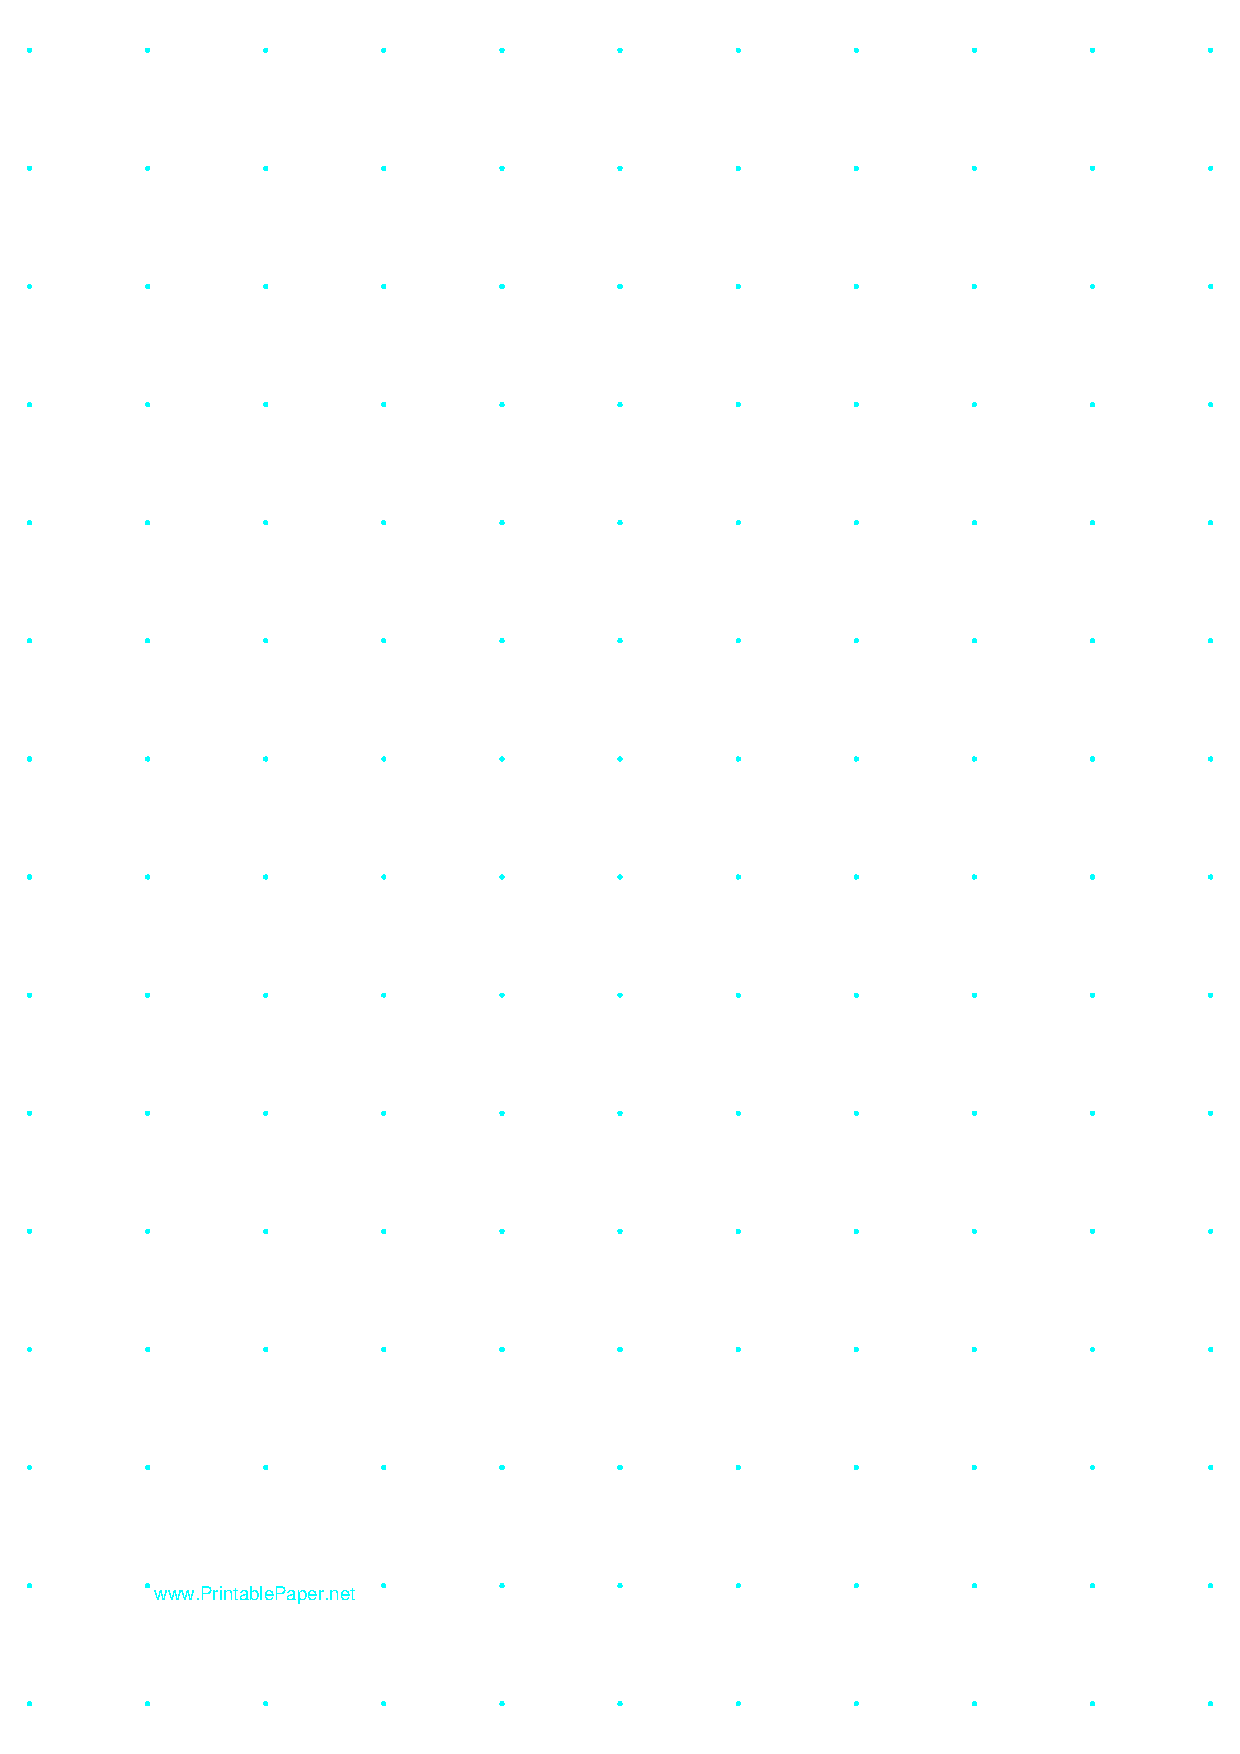
\includepdf{voorblad.pdf} 
   
\begin{songs}{}
\beginsong{'k Heb mijn wagen volgeladen}
\beginverse*
'k Heb mijn wagen volgeladen,
Vol met oude wijven;
Toen ze op de marrekt kwamen,
Begonnen zij te kijven
Nu neem ik van mijn levensdagen
Geen oude wijven meer op mijn wagen!
Hop, paardje hop!
\endverse
\beginverse*
'k Heb mijn wagen volgeladen,
Vol met oude mannen
Toen zij op de marrekt kwamen,
Gingen ze samenspannen.
Nu neem ik van mijn levensdagen
Geen oude mannen meer op mijn wagen!
Hop, paardje hop!
\endverse
\beginverse*
'k Heb mijn wagen volgeladen,
Vol met jonge meisjes
Toen zij op de marrekt kwamen,
Zongen zij als sijsjes
Nu neem ik van mijn levensdagen
Steeds jonge meisjes op mijn wagen!
Hop, paardje hop!
\endverse
\endsong
\begin{intersong}
    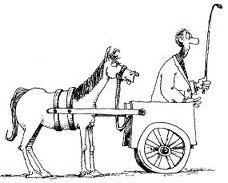
\includegraphics[width=0.4\textwidth]{img1}
\end{intersong}
\beginsong{'s Monjdoos}
\beginverse*
En 's monjdoos, tein gommen nie weirken.
En tauësjendoos gommen op zwier.
Goensjtoogs zeu zat as e veirken.
En tonderdoos spauve me zier.
Tvrauëdoos, tein gommen beginnen.
En sooëterdoos emmen geen pree.
Wa moet er ons vrauken beginnen,
me azeu ne zatte kadee?
\endverse
\beginverse*
Drinkt, drinkt, drinkt aujlen zat,
drinkt aujlen e stik in a kleuten.
Drinkt, drinkt, drinkt aujlen zat,
drinkt aujlen e stik in a gat.
\endverse
\endsong
\beginsong{'t Is welle, welle, wel}
\beginverse*
't Is welle, welle, wel, 't is wel
't Is welle, welle, wel, 't is wel
't Is welle, welle, wel,
't Is zeker wel,
't Is welle, welle, wel, 't is wel
\endverse
\endsong
\beginsong{A la claire Fontaine}
\beginverse
A la claire Fontaine
M'en allant promener,
J'ai trouvé l'eau si belle
Que je m'y suis baigné.
\endverse
\beginchorus
Il y a longtemps que je t'aime
jamais je ne t'oublierai …
\endchorus
\beginverse
Sous les feuilles d'un chêne
Je me suis fait sécher
Sur la plus haute branche
Le rossignol chantait
\endverse
\beginverse
Chante rossignol, chante
Toi qui as le coeur gai;
Tu as le coeur à rire
Moi je l'ai à pleurer.
\endverse
\beginverse
J'ai perdu mon amie
Sans l'avoir mérité
Pour un bouquet de roses
Que je lui refusai
\endverse
\beginverse
Je voudrais que la rose
Fût encore à planter
Et que ma douce amie
Fut encore à m'aimer
\endverse
\endsong
\beginsong{A ram sam sam}
\beginverse*
A ram sam sam, a ram sam sam
Goeli goeli goeli goeli
ram sam sam
Arabi , Arabi
Goeli goeli goeli goeli
ram sam sam.
\endverse
\endsong
\beginsong{Ahoelaba}
\beginverse
In d' Afrikaanse bossen, waar alle negers krossen.
Daar in die wildernis, daar woont mijn Oela Oelaba.
\endverse
\beginchorus
Ahoelaba, ik van je hou.
Ahoelaba, jij wordt mijn Afrikaanse vrouw.
\endchorus
\beginverse
Ik bloemen pluk voor Oela, maar Oela ze verkoop.
Ik Oela kusje geven, en Oela aan de loop.
\endverse
\endsong
\begin{intersong}
    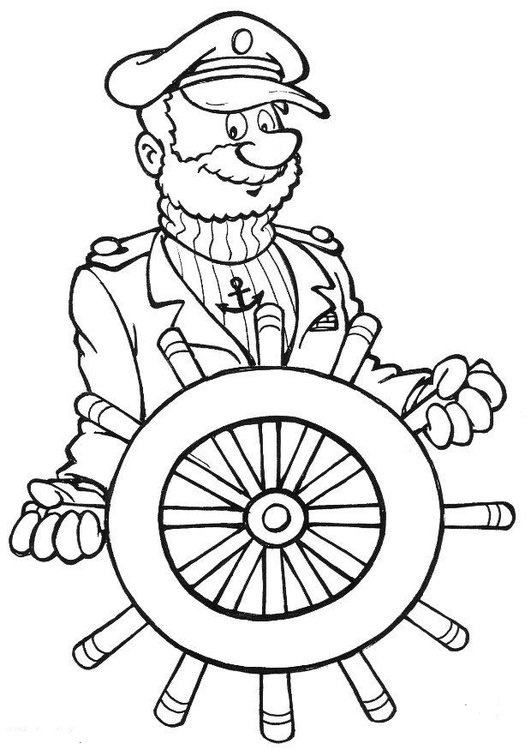
\includegraphics[width=0.4\textwidth]{img2}
\end{intersong}
\beginsong{Al die willen te kaap'ren  varen}
\beginverse*
Al die willen te kaap'ren  varen, moeten mannen met baarden zijn.
Jan, Piet, Tjores en Corneel: Die hebben baarden, die hebben baarden.
Jan, Piet, Tjores en Corneel: Die hebben baarden, zij varen mee.
\endverse
\endsong

\beginsong{Aloutte}
\beginverse
Alouette, gentille alouette, alouette, je te plumerai.
Je te plumerai la tete. 
Je te plumerai la tete et la tete.
O, alouette gentille alouette, alouette, je te plumerai.
\endverse
\beginverse
Alouette, gentille alouette, alouette, je te plumerai.
Je te plumerai le bec.
Je te plumerai le bec et le bec et la tete.
O, alouette, gentille alouette, alouette, je te plumerai.
\endverse
\beginverse
...le ne'z...et le bee...et la tete
\endverse
\beginverse
...le dos...et le nez...etc...
\endverse
\beginverse
...les pattes...et le dos...etc...
\endverse
\beginverse
 ...le cou...et les pattes...etc...
\endverse
\endsong
\begin{intersong}
    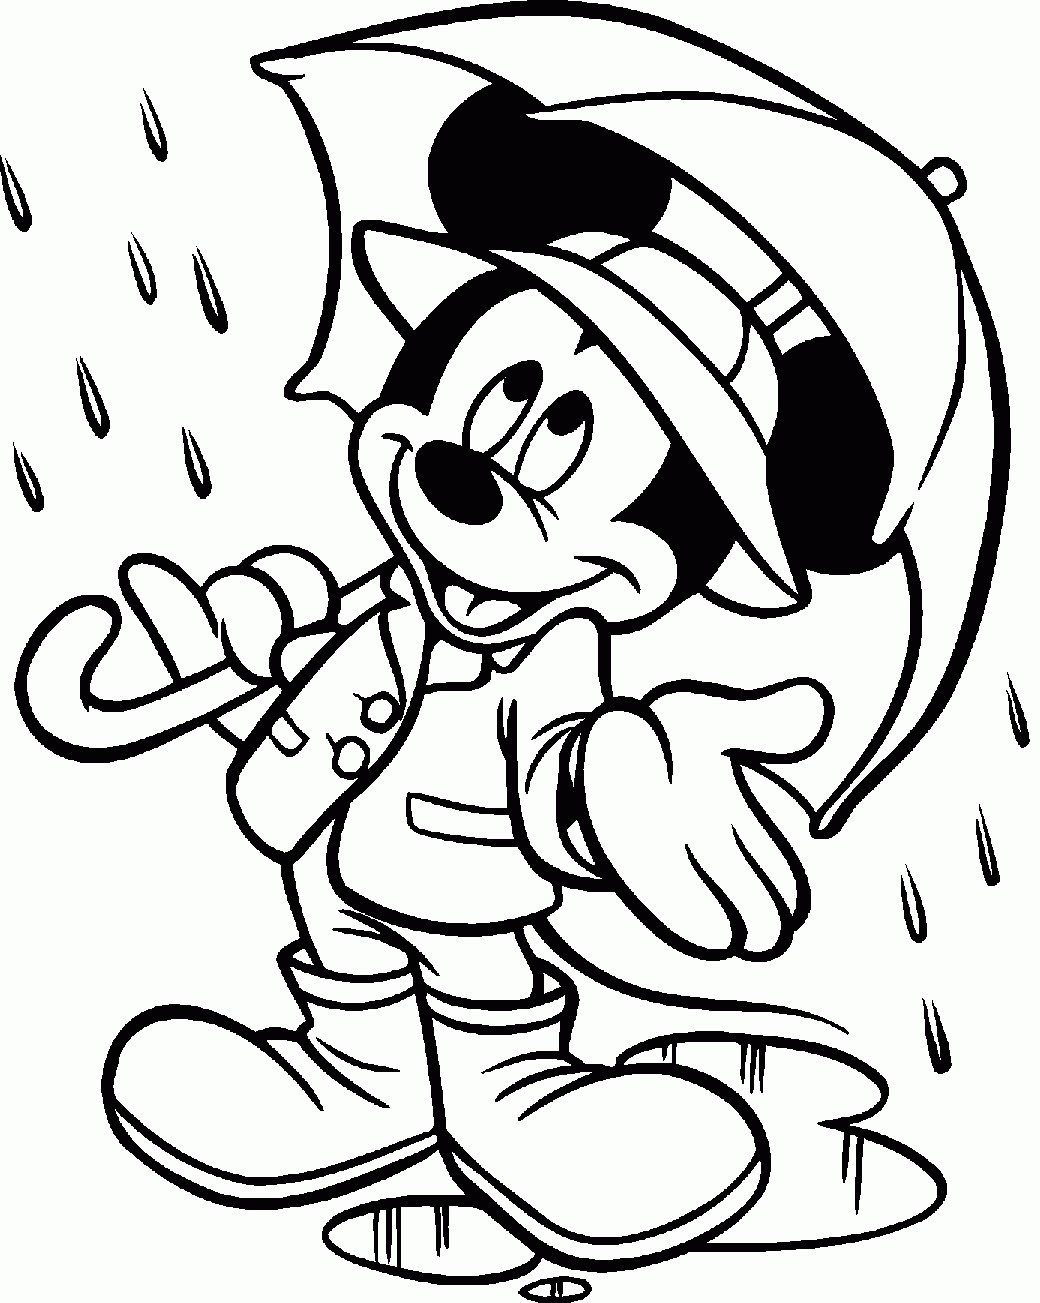
\includegraphics[width=0.4\textwidth]{deswintersalshetregent}
\end{intersong}
\beginsong{Des winters als het regent}
\beginverse
Des winters als het regent, dan zijn de paadjes diep, ja diep.
Dan komt dat loze vissertje, vissen al in dat riet, ja riet.
\endverse
\beginchorus
Met zijnen rijfstok, met zijnen strijkstok.
Met zijnen lapzak, met zijnen knapzak.
Met zijnen lere, van dirre domme dere.
Met zijne lere laarsjes aan. 
\rep{2}
\endchorus
\beginverse
Dat loze molenarinnetje, hing in heur deurtje staan, ja staan.
Opdat dat aardig vissertje, voorbij haar heen zou gaan, ja gaan.
\endverse
\beginverse
Wat heb ik u misdreven? Wat heb ik u misdaan, ja 'daan.
Opdat ik niet met vrede, vorbij uw deur mag gaan, ja gaan
\endverse
\beginverse
Gij hebt mij niets misdreven, gij hebt mij niets misdaan, ja 'daan.
Maar moet mij driemaal zoenen, eer gij van hier moogt gaan, ja gaan.
\endverse
\beginchorus
Met uwen rijfstok, met uwen strijkstok.
Met uwen lapzak, met uwen knapzak.
Met uwen lere, van dirre domme dere.
Met uwe lere laarsjes aan. 
\rep{2}
\endchorus
\endsong
\beginsong{Als de djungel}
\beginverse*
Als de djungel zich hult in het duister, flauw verlicht door het schijnsel der maan.
Sta dan stil, spits je oren en luister, zwijgend zie je de horde daar staan. 
\endverse
\beginchorus
Jalahi weerklinkt door de rimboe, 't is de kreet van het hoofd van de stam.
Alle wolven, Bagheera en Baloe, hurken neer bij de laaiende vlam. 
(En nog ne keer!)
\endchorus
\endsong
\begin{intersong}
    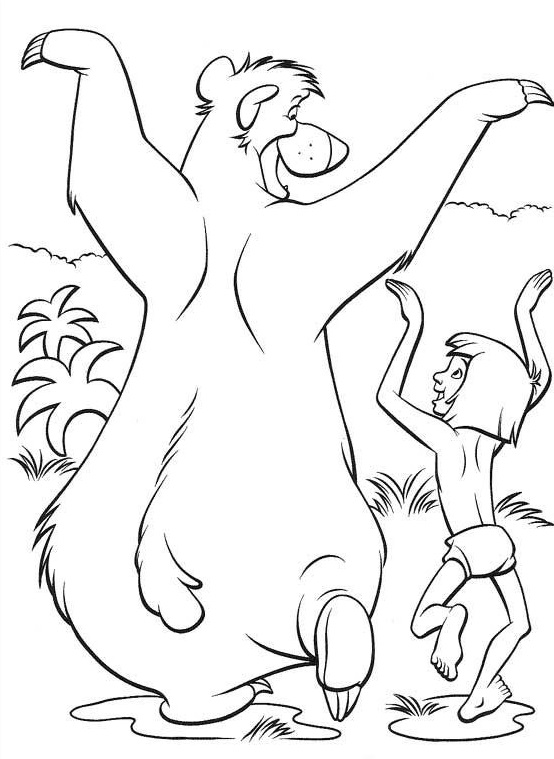
\includegraphics[width=0.4\textwidth]{img3}
\end{intersong}
\beginsong{Als de rombom}
\beginverse
Als de rombom heeft geslagen, en wij marcheren moeten gaan, geweer en ransel die moeten wij dan dragen, en dat staat ons voorwaar niet aan. 
\endverse
\beginchorus
Kapiteins en officieren, drinken wijn en soms een glaasje bier maar wij zijn maar arme fuselieren, drinken water al uit de rivier.
\endchorus
\beginverse
Een stuiver daags is onze gage, en een pondje zwart kommiezenbrood, een watersausje dat geeft ons de courage, en daarmee moeten wij dan maar voort.
\endverse
\endsong
\beginsong{Als in de mei}
\beginverse
Als in de mei, de blijde mei,
de merel fluit in 't woud,
ja fluit in 't woud,
dan trekken jonge kerels, 
van niets benauwd,
dan trekken jonge kerels, 
van niets benauwd.
\endverse
\beginchorus
Juvi valle valle valle valle lala
Juvi valle valle valle valle lala
Dan trekken jonge kerels, 
van niets benauwd.
\endchorus
\beginverse
Zij zingen luid hun lustig lied,
dat 't galme door het woud, 
ja door het woud.
Ze stappen 't leven tegen, 
van niets benauwd,
ze stappen 't leven tegen, 
van niets benauwd.
\endverse
\beginverse
Ach fiere jeugd, ach fiere jeugd,
uw lied klinkt veel te stout, 
ja veel te stout.
Ge zult wel anders zingen,
wordt gij eens oud,
Ge zult wel anders zingen,
wordt gij eens oud.
\endverse
\beginverse
Wij zingen nooit een ander lied,
al klinkt het nog zo stout,
ja nog zo stout.
Wij stoere vlaamse kerels, 
nooit worden w' oud,
wij stoere vlaamse kerels, 
nooit worden w' oud.
\endverse
\endsong
\begin{intersong}
    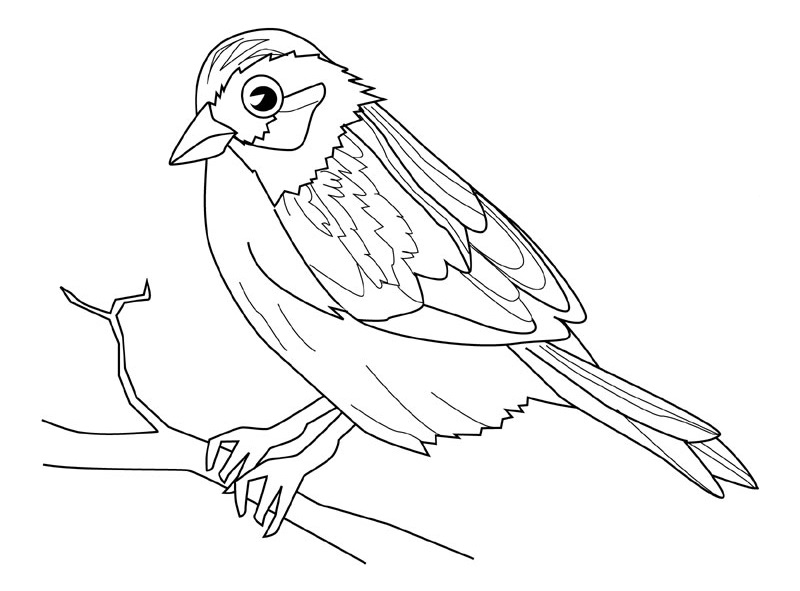
\includegraphics[width=0.4\textwidth]{img4}
\end{intersong}
\beginsong{Anne mie}
\beginverse*
Anne mie, warum hast du mir nicht geschrieben?
Anne mie, warum hast du mir nicht geschrieben?
Anne mie, und ich vergess dich nie.
Ich mag so gern, so gern nach House wiedergehn, und meine Liebste wiedersehen.
Ich mag so gern, so gern nach House wiedergehn, und meine Liebste wiedersehen.
\endverse
\beginverse*
Infanterie, du bist der schönste aller Waffen.
Infanterie, du bist der schönste aller Waffen.
Infanterie, und ich vergess dich nie...
\endverse
\endsong
\beginsong{Annemarieken}
\beginverse*
Wel Annemarieken waar ga je naartoe? \rep{2}
'k Ga naar den buiten al bij de soldaten hopsasafallala Annemarie. \rep{2}
\endverse
\beginverse*
Wel Annemarieken wat ga je daar doen? \rep{2}
Haspen en spinnen, soldaatjes beminnen hopsasafallala Annemarie. \rep{2}
\endverse
\beginverse*
Wel Annemarieken heb jij er geen man? \rep{2}
Heb ik geen man, dan krijg ik geen slagen hopsasafallala Annemarie. \rep{2}
\endverse
\beginverse*
Wel Annemarieken heb jij er geen kind? \rep{2}
Heb ik geen kind, dan moet ik niet zorgen hopsasafallala Annemarie. \rep{2}
\endverse
\endsong
\beginsong{Au clair de la lune}
\beginverse*
Au clair de la lune, mon ami Pierrot. Prete-moi ta plume pour ecrire un mot. Ma chandelle est morte, je n'ai plus de feu, ourvre-moi ta porte pour l'amour de Dieu!
\endverse
\beginverse*
Au clair de la lune,Pierrot repondit: "Je n'ai pas de plume, Je suis dans mon lit. Va chez la voisine, Je crois qu'ell y est, car dans sa cuisine on bat le briquet."
\endverse
\beginverse*
Au clair de la lune, L'aimable Lubin. Frappe chew la brune, Ell' repond soudain: "Qui frappe d'la sorte?" Il dit a son tour: "Ouvrez votre porte pour le dieu d'amour!"
\endverse
\beginverse*
Au clair de la lune, On n'y voit qu'un peu. On chercha la plume, On chercha du feu. En chercant d'la sort, Je n'sais c' qu'on trouva: Mais j'sais que la porte  sur eux se ferma.
\endverse
\endsong
\begin{intersong}
    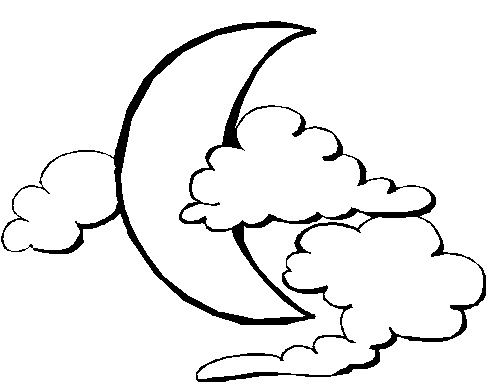
\includegraphics[width=0.4\textwidth]{img5}
\end{intersong}
\beginsong{Auprès de ma blonde}
\beginverse
Dans les jardins d'mon père, les lilas sont fleuris, tous les oiseaux du monde y viennent faire leur nid.
\endverse
\beginchorus
Auprès de ma blonde, qu'il fait bon, fait bon, fait bon.
Auprès de ma blonde, qu'il fait bon dormir.
\endchorus
\beginverse
Tous les oiseaux du monde y viennent faire leur nid, la caille, la tourtelle, et la jolie perdrix.
\endverse
\beginverse
La caille, la tourtelle, et la jolie perdrix, et ma jolie colombe, qui chante jour et nuit.
\endverse
\beginverse
Et ma jolie colombe, qui chante jour et nuit, qui chante pour les filles, qui n’ont point de mari.
\endverse
\beginverse
Qui chante pour les filles, qui n’ont point de mari, pour moi ne chante guère, car j’en ai un jolie.
\endverse
\beginverse
Pour moi ne chante guère, car j’en ai un jolie, dites-nous, donc, la belle, ou donc est votr’mari.
\endverse
\beginverse
Dites-nous, donc, la belle, ou donc est votr’mari, il est dan la Holland, les Hollandais l’ont pris.
\endverse
\beginverse
Il est dan la Hollande, les Hollandais l’ont pris, que donneriez-vous, belle, pour avoir vort’mari
\endverse
\beginverse
Qui donneriez-vous, belle, pour avoir votr’mari, je donnerais Versailles, Paris et Saint-Denis.
\endverse
\beginverse
Je donnerais Versaille, Paris et Saint-Denis, les tours de Notre-Dame et l’clocher de sons pays.
\endverse
\beginverse
Les tours de Notre-Dame et l’clocher de sons pays, et ma joli colombe, pour avoir mon ami.
\endverse
\endsong
\beginsong{Avondlied}
\beginverse
O Heer, d'avond is neergekomen. De zonne zonk, het duister klom. De winden doorruisen de bomen. En verre sterren staan alom. Wij knielen neer om U te zingen. In't slapend woud ons avondlied. Wij danken U voor wat we ontvingen. En vragen, Heer, verlaat ons niet.
\endverse
\beginchorus
Scouts en leiders knielen wij neder. Door de stilte weerklinkt onze bee. Luistrend fluistren kruinen mee. En sterren staren teder. Geef ons, Heer, zegen en rust en vree...
\endchorus
\beginverse
Gij hebt dezen dag ons gegeven. En ons bewaard gezond en blij. Uw engel is ons bijgebleven. En heeft gewandeld aan ons zij! We deden goed met uw genaden. We leerden menig wijze raad. Eenieder heeft door woord en daden. Zijn makkers broederlijk gebaat!
\endverse
\beginverse
Al wat wij boos en zwak misdeden. Vergeef het ons, O goede Heer. Uw liefde heeft voor ons geleden. Wees ons barmhartig nog een keer... Wij willen weer U trouw beloven. Ons Woord vernieuwen, Heer, voor U. En zeker van Uw hulp van boven. Laat ons gelukkig slapen nu!
\endverse
\beginverse
Weleer toen uw apostlen sliepen, toen badt G'op enen berg alleen. Waak over ons, die U aanriepen. Drijf duivel, dood en vijand heen... Waak over ons, Gij, Licht en Leven, Gij Waarheid, en 'ge Levensbaan. En morgen wordt U weer gegeven, Elke avond, ieder zonopstaan!
\endverse
\endsong
\begin{intersong}
    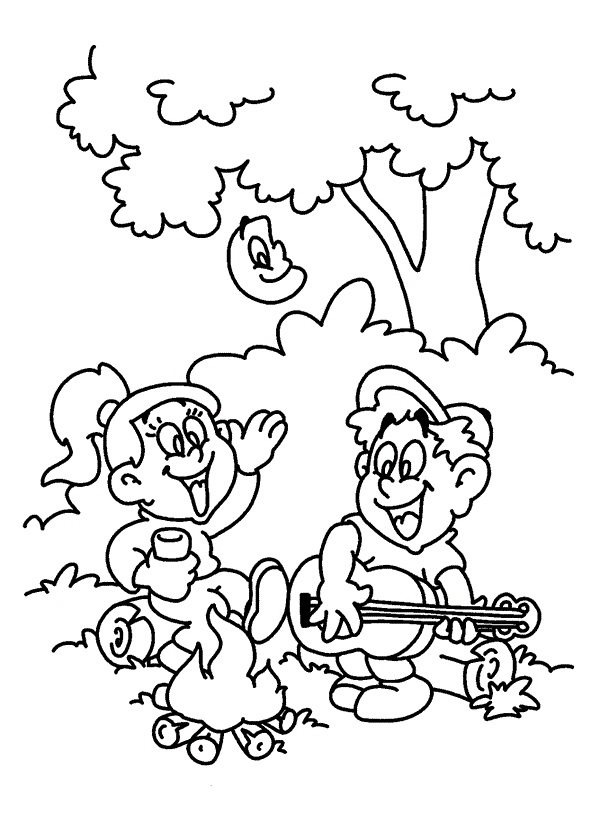
\includegraphics[width=0.4\textwidth]{img6}
\end{intersong}
\beginsong{Begroetingslied}
\beginverse*
hallo, hallo, hallo , hallo
Wij komen u groeten
Zijn blij u t'ontmoeten
hallo, hallo, hallo , hallo
\endverse
\endsong
\beginsong{Belgisch Volkslied}
\beginverse*
O dierbaar Belgie, O heilig land der vad'ren, Onze ziel en ons hart zij U gewijd.
Aanvaard ons kracht en het bloed van ons ad'ren. Wees ons doel in arbeid en in strijd.
Bloei o land, in eendracht niet te breken. Wees immer uzelf, en ongeknecht.
Het woord getrouw dat ge onbevreesd moogt spreken: Voor vorst, voor vrijheid en voor recht.
Voor vorst, voor vrijheid en voor recht.\rep{2}

\endverse
\endsong
\beginsong{Beloftelied}
\beginverse
Wij hebben u, o Jezus
Plechtig beloofd
U altijd te erkennen
Als opperhoofd.
\endverse
\beginchorus
Geef dat w'u minnen zouden
Steeds meer en meer,
Help ons belofte houden
Jezus onze Heer.
\endchorus
\beginverse
Wij hebben het gezworen
Dat Gij steeds zoudt
Ons hoofd en leider wezen
Als opperscout.
\endverse
\beginverse
Geef dat w'u minnen zouden
Steeds meer en meer,
Help ons belofte houden
Jezus onze Heer.
\endverse
\beginverse
Wij zullen gans ons leven
Lijk Gij 't geboodt
U volgen en U dienen
Tot aan ons dood.
\endverse
\beginverse
Geef dat w'u minnen zouden
Steeds meer en meer,
Help ons belofte houden
Jezus onze Heer.
\endverse
\endsong
\begin{intersong}
    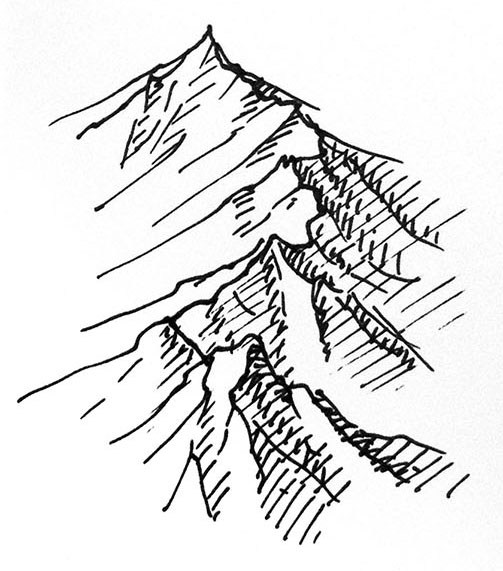
\includegraphics[width=0.4\textwidth]{bergvagebunden}
\end{intersong}
\beginsong{Bergvagebunden}
\beginverse
Wenn wir erklimmen schwindelnde Höhen,
Steigen dem Gipfelkreuz zu;
In unsern Herzen brennt eine Seesicht,
Die lässt uns nimmer mehr in ruh. 
\endverse
\beginchorus
Herrliche Berge, Sonnige Höhen,
Bergvagebunden sind wir, ja wir,
Herrliche Berge, Sonnige Höhen,
Bergvagebunden sind wir.
\endchorus
\beginverse
Mit Seil und Haken, den Tod im Nacken,
Hängen wir an der steilen Wand. 
Herzen erglühen, Edelweiß blühen,
Vorbei geht’s mit sicheren Hand.
\endverse
\beginverse
La Montanara und Puchiana,
Berge sind überall schön.
Gletscher und Sonne, Herzen voll Wonne,
Herllich die Berge zu sehn.
\endverse
\beginverse
Beim Alpenglühen heimwärts wir ziehen,
Berge, die leuchten so rot. 
Wir kommen wieder, denn wir sind Brüder,
Brüder auf Leben und Tod.
\endverse
\beginchorus
Lebwohl ihr Berge,
Sonnige Höhen,
Bergvagebunden sind treu, ja treu,
Lebwohl ihr Berge, Sonnige Höhen,
Bergvagebunden sind treu. 
\endchorus
\endsong
\beginsong{Bert Rodenbach}
\beginverse*
Bert Rodenbach die heeft een vogel in zijn hand. 
Bert Rodenbach die heeft een vogel in zijn hand.
Bert Rodenbach die heeft een vogel in zijn hand, een vogel in zijn hand. Tarara…
\endverse
\beginverse
Bert Rodenbach die heeft een vogel in zijn …
\endverse
\beginverse
Bert Rodenbach die heeft een vogel in …
\endverse
\beginverse
Bert Rodenbach die heeft een vogel …
\endverse
\beginverse
Bert Rodenbach die heeft een …
\endverse
\beginverse
Bert Rodenbach die heeft ...
\endverse
\beginverse
Bert Rodenbach die …
\endverse
\beginverse
Bert Rodenbach …
\endverse
\beginverse
Bert ...
\endverse
\endsong
\begin{intersong}
    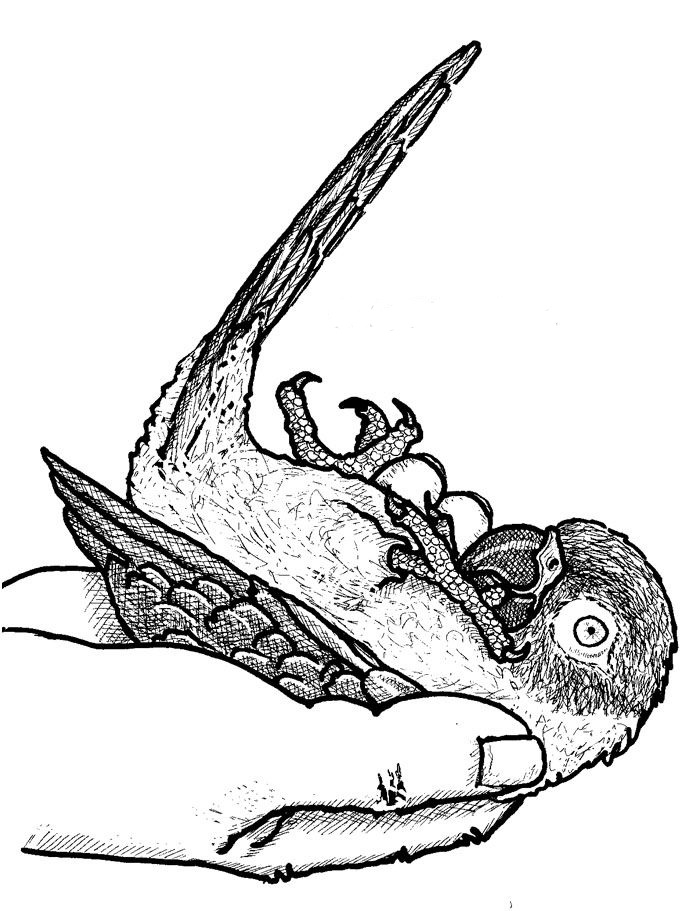
\includegraphics[width=0.4\textwidth]{bertrodenbach}
\end{intersong}
\beginsong{Bier her, Bier her}
\beginverse*
Bier her, Ber her, 
oder ich fall’um jochhe,
Bier her, Bier her,
oder ich fall’um.
Soll das BIer im Keller liegen,
und ich hier die ohnmacht kriegen,
Bier her, Bier her,
oder ich fall’um.
\endverse
\beginverse*
Bier her, Bier her,
oder ich fall’um jochhe,
Bier her, Bier her,
oder ich fall’um.
Wenn nicht gleich Bier bekumm’
schmeisz’ich ganze Kneipe um.
Bier her , Bier her,
oder ich fall’um.
\endverse
\endsong
\beginsong{Blowing in the wind}
\beginverse
How many roads must a man walk down
Before they call him a man?
How many seas must a white dove sail
Before she sleeps in the sand?
How many times must the cannonballs fly
Before they're for ever band?
\endverse
\beginchorus
The answer my friend,
Is blowin' in the wind,
The answer is blowin' in the wind.
\endchorus
\beginverse
How many times must a man look up
Before he can see the sky?
How many ears must one have
Before he can heare people cry?
How many deaths will it take till he know
That to many people had died?
\endverse
\beginverse
How many years can a mountain exist
Before he washed to the sea?
How many years can some people exist
Before they're allowed to be free?
How many times can a man turn his head
And pretend that he just doesn't see?
\endverse
\endsong
\beginsong{Brede velden}
\beginverse*
Brede velden, verre heiden,
waar ons hart zicht aan verpandt.
In uw stille, trouwe aarde,
staat zo menig kruis geplant.
In uw stille, trouwe aarde,
staat zo menig kruis geplant.
\endverse
\beginverse*
Oude fierheid, lang vergeten,
hoe lang nog blijft gij geknecht?
In ons harten, kameraden,
brandt 't vuur dat land weer recht.
In ons harten, kameraden,
brandt 't vuur dat land weer recht.
\endverse
\endsong
\beginsong{Chevaliers de la table ronde}
\beginverse
Chevaliers de la table ronde,
allons voir si le vin est bon
\endverse
\beginchorus
Allons voir, oui, oui, oui,
allons voir, non , non, non,
allons voir, si le vin est bon.
\endchorus
\beginverse
J’en boira cinq à six bouteilles,
une femme sur mes genoux.
Mais voilà qu’on frappe à la porte
je crois bien que c’est le mari.
\endverse
\beginverse
Si je meurs, je veux qu’on m’enterre,
dans une cave où il y a du bon vin.
Les deux pieds contre la muraille,
et la tête sous le robinet.
\endverse
\beginverse
Sur ma tombe je veux qu’on inscrive:
ici gît le roi des buveurs.
La morale de cette histoire,
c’est de boire avant de mourir.
\endverse
\beginverse
La morale de cette morale
c’est que les hommes sont des couchons
La morale de cette morale
c’est que les femmes aiment les couchons.
\endverse
\endsong
\beginsong{Clementine}
\beginverse
In a cavern, in a canyon,
excavating for a mine,
dwelt a miner, fortyniner, 
and his daughter, Clementine.
\endverse
\beginchorus
Oh my darling, oh my darling,
oh my darling, Clementine.
You are lost and gone forever,
dreadful sorry, Clementine.
\endchorus
\beginverse
Light she was, and like a fairy,
and her shoes were number nine,
Herring boxes, without topses,
sandals were for Clementine.
\endverse
\beginverse
Drove she ducklings to the water,
ev’ry morning, just at nine
hit her foot against a splinter,
fel into the foaming brine.
\endverse
\beginverse
Ruby lips above the water,
blowing bubbles, soft and fine,
but alas, I was no swimmer, 
so I lost my clementine.
\endverse
\beginverse
When the miner forty-niner,
Soon began to peak and pine,
Thought he oughter "jine" his daughter,
Now he's with his clementine.
\endverse
\beginverse
In a corner of the churchyard,
Where the myrtle boughs entwine,
Grow the roses in their poses,
Fertilized by Clementine.
\endverse
\beginverse
In my dreams she still doth haunt me
robed in garments, soaked in brine,
though in life I used to hug her, 
now she’s dead I draw the line.
\endverse
\beginverse
How I missed her, how I missed her
How I missed my Clementine.
So I kissed her little sister,
And forgot my Clementine.
\endverse
\endsong
\begin{intersong}
    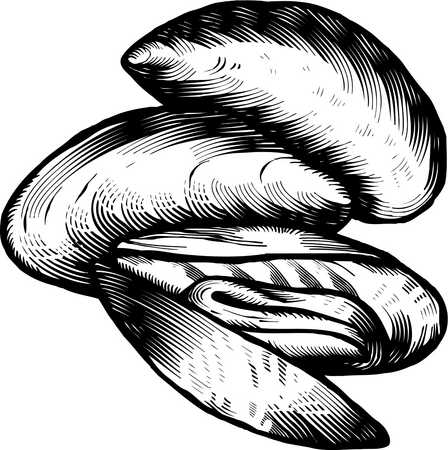
\includegraphics[width=0.4\textwidth]{cocklesandmussels}
\end{intersong}
\beginsong{Cockles and Mussels}
\beginverse
In Dublin's fair city, Where the girls are so pretty,
I first set my eyes on sweet Molly Malone,
As she wheeled her wheel-barrow,
Through streets broad and narrow,
\endverse
\beginchorus
Crying, "Cockles and mussels, alive, alive, oh!"
"Alive, alive, oh, Alive, alive, oh,"
Crying,  "Cockles and mussels, alive, alive, oh".
\endchorus
\beginverse
She was a fishmonger, But sure 'twas no wonder,
For so were her father and mother before,
And they wheeled their barrows,
Through the streets broad and narrow,
\endverse
\beginverse
She died of a fever, And no one could save her,
And that was the end of sweet Molly Malone.
But her ghost wheels her barrow,
Through streets broad and narrow,
\endverse
\endsong
\beginsong{Daar is de lente}
\beginverse*
Daar is de lente, daar is de zon,
Bijna maar ik denk dat ze weldra zal komen.
De fallus impudicus staat al in bloei,
En de blaadjes krijgen bomen. 
\endverse
\beginverse*
Mijn vrouw en mijn kat zijn allebei krols,
Het valt me moeilijk ze rustig te houden.
Ik zal binnenkort weer een heleboel
Nesten moeten bouwen. 
\endverse
\beginverse*
Want daar is de lente, daar is de zon,
Bijna maar ik denk dat ze weldra zal komen.
De fallus impudicus staat al in bloei,
En de blaadjes krijgen bomen.
\endverse
\beginverse*
De bloemknoppen barsten open met een 
Knal en de meisjes ontbloten de kuiten.
De bouwvakkers hebben na n’nare tijd
Weer iets om naar te fluiten. 
\endverse
\beginverse*
Daar is de lente, daar is de zon,
Bijna maar ik denk dat ze weldra zal komen,
De fallus impudicus staat al in bloei
En de klokken vertrekken naar Rome. 
\endverse
\endsong
\begin{intersong}
    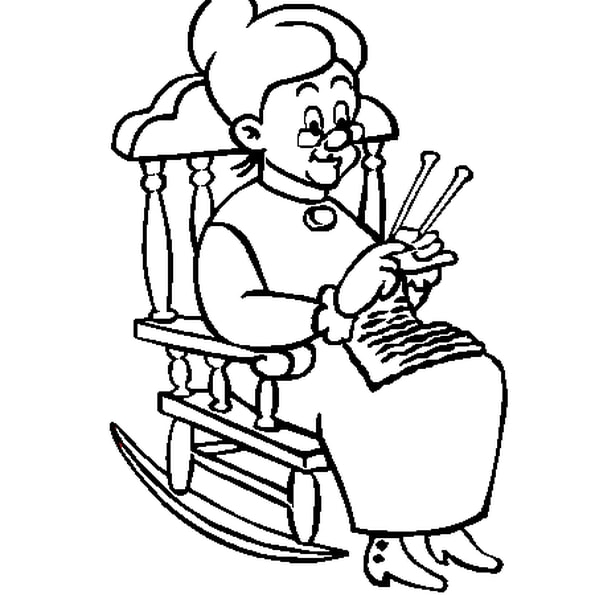
\includegraphics[width=0.4\textwidth]{daarwaseenwufdiespon}
\end{intersong}
\beginsong{Daar was een wuf die spon}
\beginverse
Daar was een wuf die spon,
Daar was een wuf die spon,
Al op een houten spinnewiel,
Daar was geen toortelten aan.
Vive la peperbusse, viva la spa, trala la la
Gize gaze gouze, ron flon flouze, traderadera!
\endverse
\beginverse
Haar mutse stoeg verdraaid,
Haar mutse stoeg verdraaid,
Gelijke een Hollands moleken,
Die met al windeken draait.
Vive la peperbusse, viva la spa, trala la la
Gize gaze gouze, ron flon flouze, traderadera!
\endverse
\beginverse
Dat wuf had enen zin,
Dat wuf had enen zin,
Als zij 's morgen buiten kroop,
's Avonds dan kroop zij er in. 
Vive la peperbusse, viva la spa, trala la la
Gize gaze gouze, ron flon flouze, traderadera!
\endverse
\beginverse
3.	Dat wuf had enen man,
Dat wuf had enen man,
's Zondags heet hij Pieter,
's Maandags heet hij Jan. 
Vive la peperbusse, viva la spa, trala la la
Gize gaze gouze, ron flon flouze, traderadera!
\endverse
\endsong
\beginsong{Daar was laatst een meisje loos}
\beginverse
Daar was laatst een meisje loos, 
Die wou gaan varen,
Die wou gaan varen,
Daar was laatst een meisje loos,
Die wou gaan varen als lichtmatroos.
\endverse
\beginverse
Zij moest klimmen in de mast,
Maken de zeilen,
Maken de zeilen,
Zij moest klimmen in de mast,
Maken de zeilen met touwtjes vast.
\endverse
\beginverse
Maar door storm en tegenweer,
Sloegen de zeilen,
Sloegen de zeilen,
Maar door storm en tegenweer,
Sloegen de zeilen van boven neer. 
\endverse
\beginverse
“Och, kapiteintje, sla me niet,
Ik ben uw liefje,
Ik ben uw liefje,
Och, kapiteintje, sla me niet,
Ik ben uw liefje zoals gij ziet.”
\endverse
\beginverse
Zij moest komen in de kajuit,
Kreeg een pak ransel,
Kreeg een pak ransel,
Zij moest komen in de kajuit,
Kreeg een pak ransel en toen was 't uit. 
\endverse
\endsong
\beginsong{ Daar zat een sneeuwwit vogeltje}
\beginverse*
Daar zat een sneeuwwit vogeltje (bis)
Al op een stelceldorentje, din don deine!
Al op een stelceldorentje, din don don.
\endverse
\beginverse*
" Wilt gij niet mijnen bode zijn? " (bis)
" Ik ben te klein een vogelkijn, din don deine ” 
" Ik ben te klein een vogelkijn, din don don. "
\endverse
\beginverse*
" Zijt gij maar kleine, gij zijt snel; (bis)
“Gij weet den weg? " " Ik weet hem wel, din don deine!”
“ Gij weet den weg? " " ik weet hem wel, din don don. ”
\endverse
\beginverse*
Hij nam den brief in zijnen bek (bis)
En vloog er mee tot over 't hek, din don deine.
En vloog er mee tot over 't hek, din don don.
\endverse
\beginverse*
Hij vloog tot aan mijn zoet liefs deux: (bis)
" En slaapje of waakje, of zijt ge dood, din don deine? »
" En slaapje of waakje, of zijt ge dood, din don don."
\endverse
\beginverse*
" 'k En slape noch 'k en wake niet " (bis)
" Ik ben getxouwd al een half jaar, din don deine."
" Ik ben getrouwd al een half jaar, din don don. "
\endverse
\beginverse*
" Zijt gij getrouwd ai een half jaar? " (bis)
" Het dochte mij wel duizend jaar, din don deine. "
" Het dochte mij wel duizend jaar, din don don. "
\endverse
\endsong
\beginsong{Dank U}
\beginverse*
Dank U, voor deze nieuwe zorgen
Dank U, voor deze nieuwe dag
Dank U dat ik met al mijn zorgen
Bij U komen mag. 
\endverse
\endsong
\begin{intersong}
    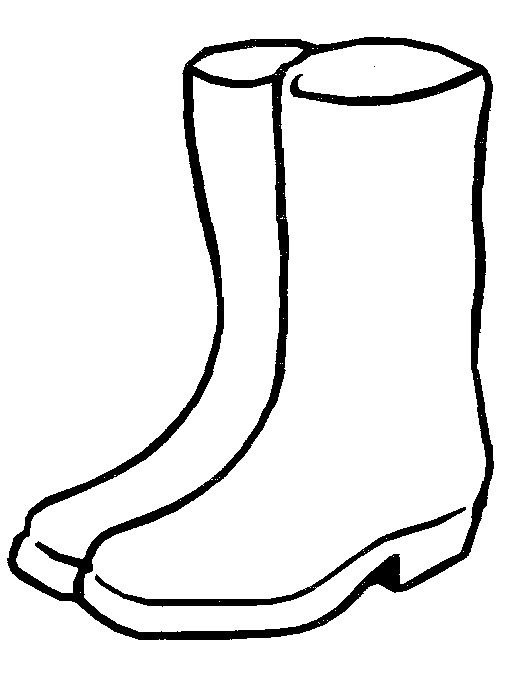
\includegraphics[width=0.4\textwidth]{deboerhadmaarenenschoen}
\end{intersong}
\beginsong{De boer had maar enen schoen}
\beginverse
De boer had maar enen schoen,
Weinig genoeg, genoeg, genoeg!
De boer had maar enen schoen,
Weinig genoeg! 
Een schoen zonder hak er an,
De boer is geen edelman,
Een schoen zonder hak er an,
De boer is geen edelman,
\endverse
\beginverse
De boer had maar enen broek: …
Een broek zonder zak erin, …
\endverse
\beginverse
De boer had maar enen jas: …
Een jas zonder knoop er an, …
\endverse
\beginverse
De boer had maar enen kous: …
Een kous met een gat er in, …
\endverse
\beginverse
De boer had maar enen hemd: …
Een hemd zonder slip er an, …
\endverse
\beginverse
De boer had maar enen pet: …
Een pet zonder klep er an, …
\endverse
\beginverse
De boer had maar enen vrouw,
Meer dan genoeg, genoeg, genoeg! 
De boer had maar enen vrouw,
Meer dan genoeg!
Een vrouw met een kop er op: 
De boer had een reuzestrop;
Een vrouw met een kop er op:
De boer die had een reuzestrop. 
\endverse
\endsong
\beginsong{De boom stond op de bergen}
\beginchorus
En de boom stond op de bergen hali-halo \rep{2}
En aan die boom daar kwam een tak,
Een reuzetak, een pracht van een tak;
Ach jongens wat een tak was dat.
De tak van de boom
En de boom stond op de bergen hali-halo \rep{2}
\endchorus
\beginverse
En aan die tak daar kwam een blad.
\endverse
\beginverse
En aan dat blad daar kwam een nest. 
\endverse
\beginverse
En in dat nest daar kwam een ei.
\endverse
\beginverse
En uit dat ei daar kwam een jong. 
\endverse
\beginverse
En aan dat jong daar kwam een veer. 
\endverse
\beginverse
En aan die veer daar kwam een hoed. 
\endverse
\beginverse
En aan die hoed daar kwam een juf. 
\endverse
\beginverse
En aan die juf daar kwam een heer. 
\endverse
\beginverse
En aan die heer daar kwam een huis.
\endverse
\beginverse
En aan dat huis daar kwam een stal.
\endverse
\beginverse
En in die stal daar kwam een geit.
\endverse
\beginverse
En aan die geit daar kwam een staart. 
\endverse
\beginverse
En aan die staart daar kwam een eind. 
\endverse
\endsong
\beginsong{De gilde viert}
\beginverse
De gilde viert, de gilde juicht,
wat zijt gij daar en blokt en buigt
nog over uwe boeken?
de wijsheid ligt maar in de kan,
die ze elders zoeken wil, die kan,
doch laat hem, laat hem zoeken.
\endverse
\beginchorus
Het beste biertjes lust hij niet,
het liefste liedje sust hem niet,
het mooiste meisje kust hij niet,
hoog het glas, hoog het hart, hoog het bier.
\endchorus
\beginverse
De beker ruist, de beker schuimt,
sa makkers fris en opgeruimd,
het glas aan uwe lippen,
die op zijn kamer koekeloert,
en gestversnip’rend dwaasheën snoert,
drinkt water als de kippen.
\endverse
\beginverse
Het pijpke dampt in nonkelmond,
en spreidt wellustig in het rond,
studentikoze geuren.
Die steeds aan perkamenten kluift,
en perkamenten reuken snuift,
krijgt perkamentenkleuren.
\endverse
\beginverse
De gilde juicht, de gilde viert,
hoera, de pet omhoog gezwierd,
en nog eens hard geklonken.
De blokker ligt reeds log en loom,
gekweld door nare blokkersdroom,
met droge keel te ronken.
\endverse
\endsong
\beginsong{De Jef van de Capucienen}
\beginverse
En de Jef van de Capucienen \rep{2}
En de Capucienen Jef		
Larie tsjoemlalalalalaliere… \rep{2}
\endverse
\beginverse*
Jef = pssst
Jef = hum
Jef = fwiet (fluiten)
Jef = klop (op tafel)
Jef = knip (met vingers)
Jef = oogje trekken
\endverse
\endsong
\begin{intersong}
    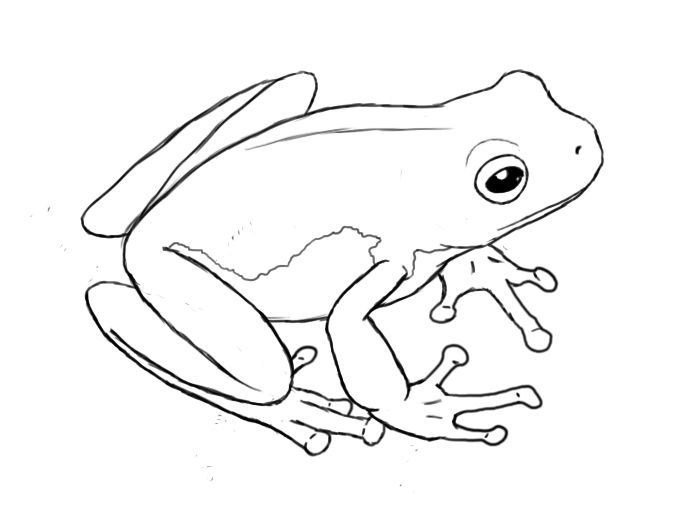
\includegraphics[width=0.4\textwidth]{dekikker}
\end{intersong}
\beginsong{De Kikker}
\beginverse
Aan den oever van de Dijle,
Diep verscholen in het riet,
Zat een kleine jonge kikker
Bij zijn moeder op de knie!
\endverse
\beginverse
"Ziet ge daar" zo sprak die moeder,
"Ziet ge daar dien ooievaar,
't Is de moord'naar van uw vader,
Hij vrat hem op met huid en haar".
\endverse
\beginverse
"Godverdomme", sprak die kleine,
"Heeft die smeerlap dat gedaan,
Als ik groot en sterk zal wezen
Zal op op zijn bakkes slaan"!
\endverse
\beginverse
Vele jaren zijn verstreken,
En de kikker leeft niet meer.
Maar de ooievaar die leeft nog,
En zijn bakkes doet nog zeer.
\endverse
\beginverse
'kHeb zoveel u nog te zeggen
Haar ge zoudt het niet verstaan
'k Zal u in uw bedje leggen..."
En daarmee is 't lied gedaan.
\endverse
\endsong
\beginsong{De Kikkertjes}
\beginverse
De kikkertjes, de kikkertjes
zijn aardig om te zien          
ooh, kwak-kwak-kwak… \rep{2}
\endverse
\beginchorus
In 't hoge gras, in 't lage gras
daar springen zijn in 't rond  
ooh, kwak-kwak-kwak… \rep{2}
\endchorus
\beginverse
En moederpuit, en vader puit
die gingen samen uit              
ooh, kwak-kwak-kwak… \rep{2}
\endverse
\beginverse
Scheu weer geweest, scheu weer geweest,
et ee vandoog scheu weer geweest \rep{2}
\endverse
\beginverse
et ee vandoog, scheu weer geweest 
\endverse
\beginverse
Scheu weer geweest, scheu weer geweest,
Et ee vandoog scheu weer geweest. 
\endverse    
\endsong   
\beginsong{De maanden}
\beginverse*
En al wie in de maand … geboren is, sta op!
En al wie in de maand … geboren is, sta op!
\endverse
\beginchorus
 (Als er niemand recht staat)
't Is mis, 't is mis, 't is mis.
't Is mis, 't is mis, 't is mis.
\endchorus
\beginchorus
Zet het glaasje aan je lippen,
laat het zachtjes binnenglippen.
Zet het glaasje aan je mond,
en drink het leeg.\rep{12}
\endchorus
\beginverse*
En al wie niet geboren is, sta op!
En al wie niet geboren is, sta op!
\endverse
\beginverse*
(Als er wel iemand recht staat)
Zet het glaasje aan je lippen,
laat het zachtjes binnenglippen.
Zet het glaasje aan je mond,
en drink het leeg.
\endverse
\endsong
\beginsong{De poes van tante Loes}
\beginverse*
Er is een 1,2 ,3 , 4 ,5 , 6 ,7-ling geboren, bij de
poes van tante Loes;
Er is een 1,2 , 3 , 4,5, 6, 7-ling geboren, bij de
poes van tante Loes.
Het eerste was een jongen, het tweede was een meisje,
het derde kon niet komen want het vierde was niet thuis,
het vijfde was te mager, het zesde was te dik,
en het zevenste had de poten van het achtste ingeslikt. 
Ouwe taaie...
\endverse
\endsong
\begin{intersong}
    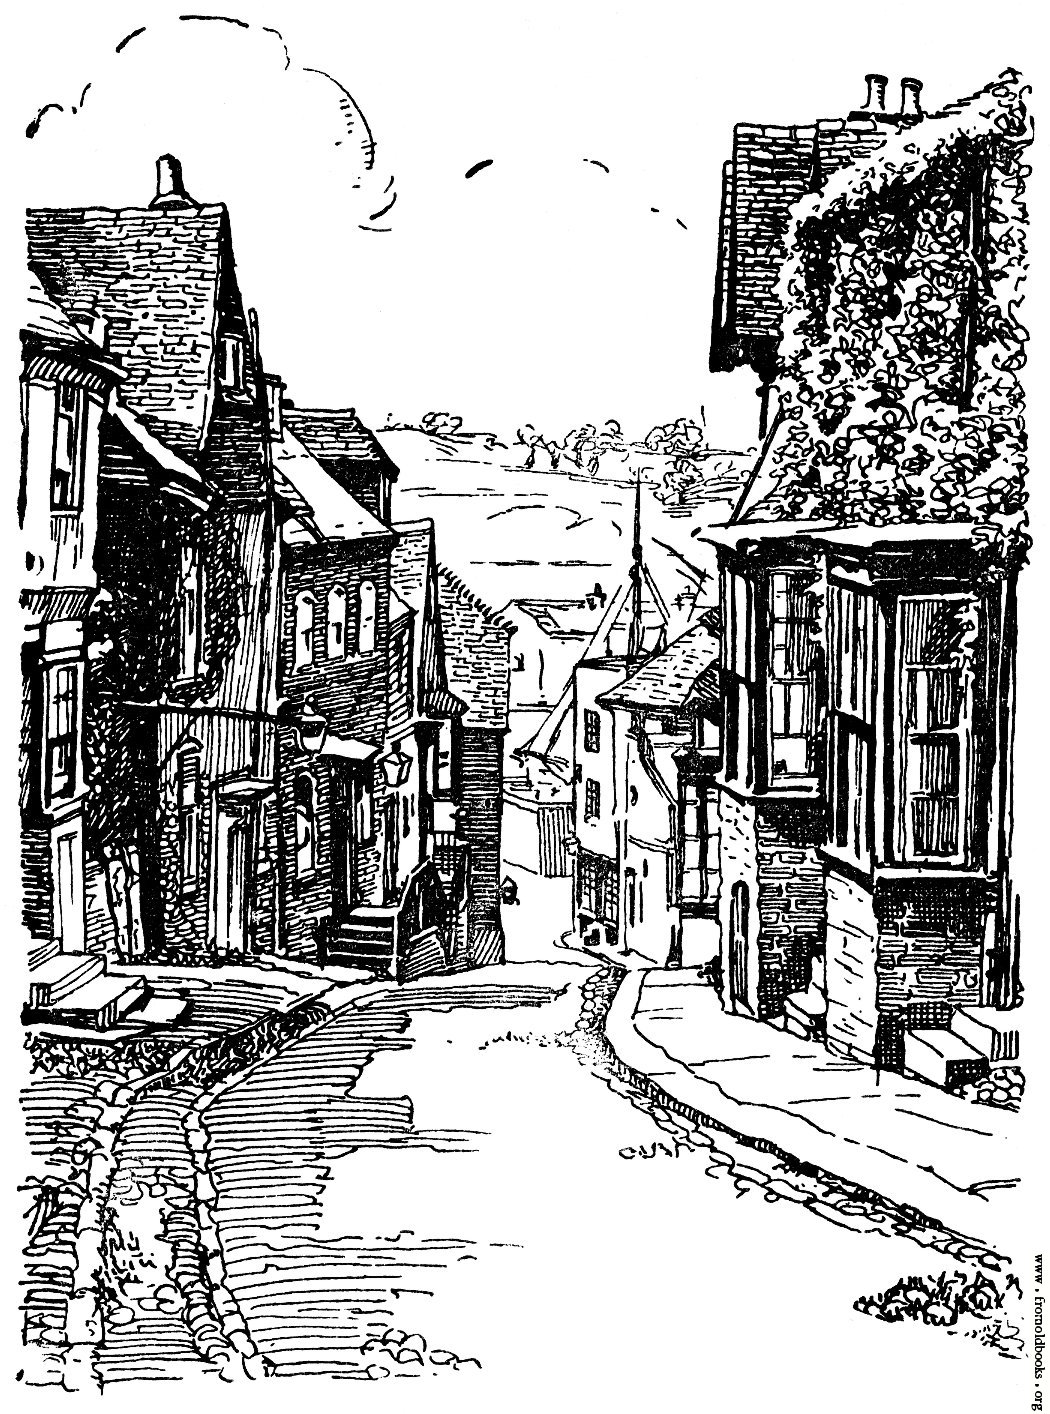
\includegraphics[width=0.4\textwidth]{destratenzijdreunen}
\end{intersong}
\beginsong{De straten zij dreunen}
\beginverse*
De straten zij dreunen bij 't schrijden,
Zo koel waait de morgenwind,
Vooraan steeds het vaandel dat wappert,
Vooraan waar het doel zich bevindt.
\endverse
\beginchorus
En schijnt ook daarboven, De hemel zo grauw;
Boven de wolken, Blijft 't eeuwig blauw.
\endchorus
\beginverse*
Wij willen de laagheid verderven,
Wij dromen van trouw en van eer,
De wereld zij mag ons onterven,
Ons stappen zij keren niet weer.
\endverse
\beginverse*
Wij zullen geen roem ons verwerven,
Maar hoog boven laster en haat,
Staat stralend geplant op de scherven,
Het vaandel dat nimmer vergaat.
\endverse
\endsong
\beginsong{De vier weverkes}
\beginverse*
Vier weverkens zag men ter botermarkt gaan, en de boter die was er zo diere.
Zij hadden geen duit haast meer in hunne tas, en ze kochten 1 pond sa vieren.
\endverse
\beginverse*
Schietspoele, sjerrebekke spoelza! Djikke djakke kerrekoltjes klitsklet
En ze kochten 1 pond sa vieren.
\endverse
\beginverse*
En als zij dat boterken hadden gekocht, zij hadden er vier platelen.
Zij spraken dat vrouwken zo vriendelijk aan: sa vrouwke en wilt het ons dele
\endverse
\beginverse*
Dat vrouwken dat sprak: Ja dat zal ik wel doen,
ja zo wel als een vrouwken vol eren
want ik wete wel wat er de weverkens zijn: en de weverkens zijn er geen her;
Wat zouden de weverkens heren zijn, zij en hebben er huize noch erven!
En kruipt er een muisken in hunne schapraai, van honger zo moet het er strerven
\endverse
\beginverse*
En als dan dat muisken gestorven zal zijn, waar zullen zij het begraven?
Al onder de weverkens hunne getouw en het grafken zal rooskens dragen.
\endverse
\endsong
\beginsong{De Vlaamse Leeuw}
\beginverse*
Zij zullen hem niet temmen, 
de fiere Vlaamse Leeuw,
Al dreigen zij zijn vrijheid,
met kluisters en geschreeuw.
Zij zullen hem niet temmen
\endverse
\beginverse*
zolang een Vlaming leeft,
Zolang de Leeuw kan klauwen, 
zolang hij tanden heeft.
Zij zullen hem niet temmen,
zolang een Vlaming leeft,
Zolang de Leeuw kan klauwen, 
zolang hij tanden heeft.
Zolang de Leeuw kan klauwen,
zolang hij tanden heeft.
\endverse
\beginverse*
De tijd verslindt de steden, 
geen tronen blijven staan:
De legerbenden sneven, 
een volk zal nooit vergaan.
De vijand trekt te velde, 
omringd van doodsgevaar.
Wij lachen met zijn woede, 
de Vlaamse Leeuw is daar
\endverse
\beginverse*
Zij zullen hem niet temmen,
zolang een Vlaming leeft,
Zolang de Leeuw kan klauwen, 
zolang hij tanden heeft.
Zolang de Leeuw kan klauwen, 
zolang hij tanden heeft.
\endverse
\beginverse*
Hij strijdt nu duizend jaren,
voor Vlaandrens dierbaar lot,
en nog zijn zijn krachten,
in al haar jeugdgenot.
Als zij hem machtloos denken,
en tergen met een schop,
dan richt Hij zich bedreigend
en vreselijk voor hen op.
\endverse
\endsong
\beginsong{Den tandem}
\beginverse*
'k Hem ver ma liefken nen tandem gekocht,
't Es plezierig rijden en we leggen ons in den bocht. 
We rijden naar den buiten, ver van de stad,
Weg van de fabrieken, en recht in 't boerengat.
\endverse
\beginverse*
Eens daar aangekomen, op de groene wei,
De bloemekes die bloeien, de boerkes die zijn blij.
Dan fluistert z’in mijn oor: kom eens dichterbij,
Geef me ne kus, geeft er mij twee, geeft er mij drei. 
\endverse
\beginverse*
We eten boerenbrood, met witte en zwarte trippen,
't Es potverdekke ver an kinne van af te likken,
We spoelen alles deure, met grote potte bier,
Geeft er mij twee, geeft er mij drei, geeft er mij vier. 
\endverse
\beginverse*
We slapen op de schelf, onder 't warme stro,
Ik en mijn liefken en heure velo,
We vragen veur nen nacht te blijven on den boer zijn wijf,
Ze zeit: blijft er mor drei, blijft er mor vier, blijft er mor vijf. 
\endverse
\beginverse*
Mor eens is 'n tijd gekomen, om naar huis te gaan,
We komen van ons schelfken en we doen ons kleren aan,
En terwijl we ons veloken gaan pakken, zei ze tegen mij,
Zouden we ons broeiken hier nie bakken?
\endverse
\beginverse*
'k Hem ver mij liefken een schelfken gekocht,
't Es plezierig vrijen en we leggen ons in den bocht,
En hier op den buiten, ver van de stad,
Spelen al onze kindjes buiten \rep{2}
Met witte en zwarte trippen  \rep{2}
En veur ons deur ligt er een mat. 
\endverse
\endsong
\beginsong{Der Pappenheimer}
\beginverse*
Wir trinken
Einen Halben in der Welt.
Warum sollten wir nicht trinken einen Halben,
Einen halben in der Welt?
General Pappenheim 
Der soll leben           
General Pappenheim
Der lebe hoch.             
Bei Wein und bei Bier,
Lustige Pappenheimer sind wir hier;
Bei Bier und bei Wein,
Lustige Pappenheimer wollen wir sein. 
\endverse
\beginchorus
“Einen Halben in der Welt” wordt bij het herhalen van het lied vervangen door wat volgt (naar keuze kan men nog aanvullen)
\endchorus
\beginverse*
Einen Halben auf dem Stuhl.
Einen Halben auf dem Tisch. 
Einen Halben unterm Tich...
\endverse
\endsong
\begin{intersong}
    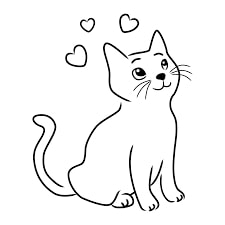
\includegraphics[width=0.4\textwidth]{diekatkomweer}
\end{intersong}
\beginsong{Die kat kom weer}
\beginverse
Die boer die zwoer hem blau: hij zou die kat doodskiet,
hij heeft die roer gelaän met kruid en dynamiet;
Hij lei hem op de weg waardoor die kat moes kom;
Haren en velletjes en beentjes.
\endverse
\beginchorus
Maar die kat kom weer, die kon nie langer wach,
die kat kom weer, die volgende dag.
Die kat kom weer, geloof me het is waar,
die volgende dag is die kat weer daar.
\endchorus
\beginverse
Hij zet hem op een skip, die zeilde naar Japan,
die skip was gelaän met twalefhonderd man.
Maar verre van die land, daar is die skip gestrand;
En alle passagiers verdronken.
\endverse
\beginverse
Die boer die zat die kat in een aëroplaan,
die botste eventjes tegen een wolkie aan.
Die boel die viel omlaag, bleef teken in een haag!
Alleman brak nek en benen.
\endverse
\beginverse
Die boer die bond die kat die pootjes netjes saam,
en lei die beesjie op de railtjes van de tram.
Die trampie liep van spoor, en brak te midden door:
stukken glas en hout en ijzer!
\endverse
\beginverse
Toen kap die boer die kat in duizend stuk kif kaf, 
en steek dan ieder stuk apaartjes in’n graf.
Hij stamp die boel goed aan en dank: het is gedaan.
Maar als hij sliep dan droomde hij altijd. 
\endverse
\endsong
\beginsong{Die Lore}
\beginverse
Im Wald, im grünen Walde,
Da steht ein Försterhaus.
Im Wald, im grünen Walde,
Da steht ein Försterhaus.
Da schauet jeden Morgen
So frisch und frei von Sorgen
Des Försters Töchterlein hinaus,
Des Försters Töchterlein hinaus.
\endverse
\beginchorus
Tiralala tiralala
Tiralala tiralala
Tira tira tiralalalala.
Tiralala tiralala
Tiralala tiralala
Tira tiralalalala.
Lore, Lore, Lore, Lore
Schön sind die Mädel von siebzehn, achtzehn Jahr.
Lore, Lore, Lore, Lore
Schöne Mädel gibt es überal.
Und kommt der Früling in das Tal
Grüsst mir die Lore noch einmal
Adee, adee adee
Und kommt der Früling in das Tal
Grüsst mir die Lore noch einmal
Adee, adee adee.
\endchorus
\beginverse
Der Förster und die Tochter
Die schossen beide gut,
Der Förster und die Tochter
Die schossen beide gut :
Der Förster schoss ein Hirchelein
Die Tochter traf ein Burchelein
Tief in das junge Herz hinein,
Tief in das junge Herz hinein.
\endverse
\endsong
\beginsong{Die Lorelei}
\beginverse*
Ich weiss nicht was soll es bedeuten
Dass ich so traurig bin,
Ein Märchen aus uralten Zeiten,
Das kommt mir nicht aus dem Sinn.
Die Luft ist kühl und es dunkelt
und ruhig fliesst der Rhein.
Der Gipfel des Berges funkelt,
Im Abendsonneschein.
\endverse
\beginverse*
Die schönste Junfrau sitzet,
Dort oben wunderbar,
Ihr goldnes Geschmeide blitzet,
Sie kämmt ihr goldnes Haar,
Sie kämmt es mit goldenem Kamme
Und singt ein Lied dabei.
das hat eine wundersame,
Gewaltige Melodie. 
\endverse
\beginverse*
Den Schiffer im kleinen Schiffe,
Ergreift es mit wilden Weh.
Er schaut nicht die Felsenriffe.
Er schaut nur hinauf in die höh.
Ich glaube die Wellen verschlingen,
Am ende Schiffer und Kahn, 
Und das hat mit ihrem singen,
Die Lorelei getan.
\endverse
\endsong
\begin{intersong}
    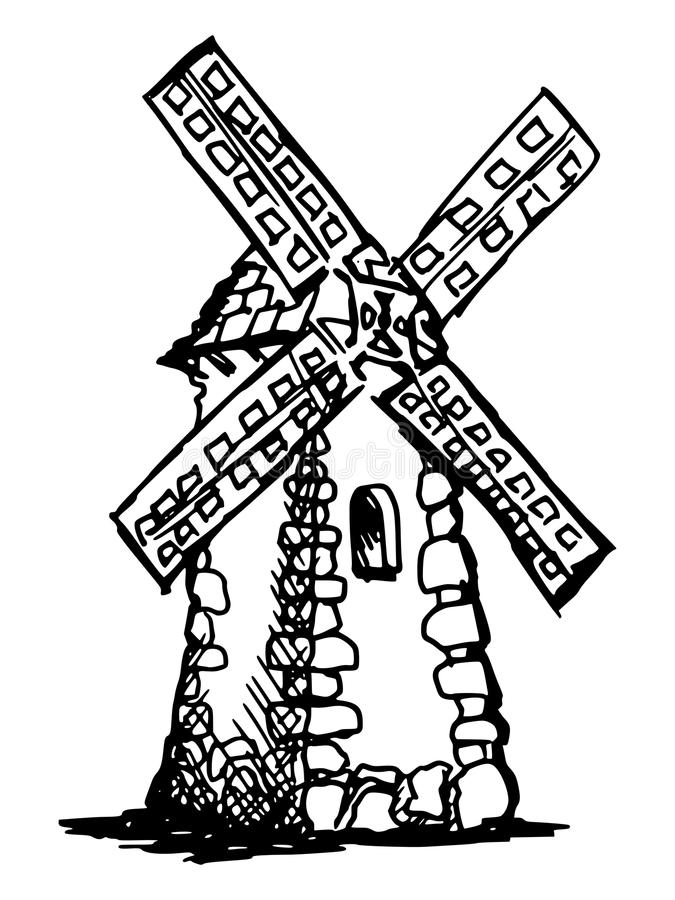
\includegraphics[width=0.4\textwidth]{diemooiemolen}
\end{intersong}
\beginsong{Die mooie molen}
\beginverse
Ik weet een heerlijk plekje grond, alwaar een molen staat,
waar ik mijn allerliefste vond, waarvoor mijn harte slaat.
Ik zag haar voor de eerste keer aan d’oever van de vliet, 
en sinds die tijd kom ik daar weer, die plek vergeet ik niet.
\endverse
\beginchorus
Daar bij die molen, die mooie molen,
daar woont een meisje waar ik zoveel van hou.
Daar bij die molen, die mooie molen,
daar wil ik wonen als jij een wordt mijn vrouw.
\endchorus
\beginverse
Als in de stille avondstond de zon ten onder ging,
en ik haar bij die molen vond in zoete mijmering,
fluisterde zij me in het oor hoe heerlijk saam te zijn.
De molen draaide lustig door en 'k zie “mijn liefste mijn”.
\endverse
\beginverse
Ik zie de molen al versierd ter eer van 't jonge paar,
en heel het dorp dat juicht en viert “zij leven menig jaar”.
En zie ik trots de molen staan, dan zweer ik in die stond,
nooit ga ik van die plek vandaan, waar ik mijn vrouwtje vond.
\endverse
\endsong
\beginsong{Door eenzelfde wet}
\beginverse*
Door eenzelfde wet steeds verbonden,
in vaste geslotene rij,
daar trekken die oude gezichten,
nog eenmaal mijn ogen voorbij.
Ik heb u eenmaal als makker zien strijden,
't vuur in d’ogen en stralend blijgemoed.
Vastbesloten om dapper te strijden,
ach wie weet wat het leven soms doet.
Maar eenmaal vind ik bij 't kruisen der wegen,
schone jeugd ach wat keer jij niet weer.
Wijl een groet komt van ver mij tegen,
mijne oude patrouilleleiders weer.
\endverse
\endsong
\beginsong{Drie shuintamboers}
\beginverse
Drie schuintamboers, die kwamen uit het Oosten, 
Van rombom, wat maal ik erom?
Die kwamen uit het Oosten.
Rombom!
\endverse
\beginverse
Een van de drie, zag daar een aardig meisje, \rep{2}
Van rombom, wat maal ik erom?
Zag daar een aardig meisje.
Rombom!
\endverse
\beginverse
Zeg meisje lief, mag ik met jou verkeren? \rep{2}
Van rombom, wat maal ik erom?
Mag ik met jou verkeren?
Rombom.
\endverse
\beginverse
Zeg jonge man, dat moet je vader vragen.
\endverse
\beginverse
Zeg ouwe heer, mag ik je dochter trouwen?
\endverse
\beginverse
Want zij is mij, de schoonste aller vrouwen.
\endverse
\beginverse
Zeg jongeman, zeg mij wat is jouw rijkdom?
\endverse
\beginverse
Mijn rijkdom is, een trommel met twee stokken.
\endverse
\beginverse
Neen schuintamboer, mijn kind kunt gij niet krijgen.
\endverse
\beginverse
Zeg ouwe heer, ik heb nog iets vergeten.
\endverse
\beginverse
Mijn vader is, Groothertog van Brittanje.
\endverse
\beginverse
Mijn moeder is, de Koningin van Spanje.
\endverse
\beginverse
Zeg jonge man, je mag mijn dochter trouwen.
\endverse
\beginverse
Neen ouwe heer, je mag je dochter houwen.
\endverse
\endsong
\beginsong{Ecce milites}
\beginverse*
Ecce mili milites Romani
Romani milites fortes
pugna pugna, pugna pugna turi
ecce nos milites 
avae Caesar, avae avae Caesar
morituri turi te salutant
adeamus pulchram machiem
\endverse
\beginverse*
Et hostes periant
adeamus pulchram machiem
et hostes periant
ecce mili milites Romani
Romani milites fortes
pugna pugna, pugna pugna turi
ecce nos milites
\endverse
\beginverse*
Avae Caesar, avae avae Caesar
morituri turi te salutant
ecce milites Romanos
Romanorum milites fortes.
\endverse
\endsong
\beginsong{Een scout dat is een jongen}
\beginverse
Een scout dat is een jongen
Gezond en weltevree.
Die zingt uit volle longen,
Met al zijn makkers mee:
\endverse
\beginchorus
En onze leuze klinkt wees vaardig
Want het leven is een strijd
Maar wij vinden ’t leven aardig 
Evenwel zijn wij bereid
\endchorus
\beginverse
De natuur is onze woning,
Daar gaan wij hand in hand
Ten strijde met de koning,
Voor God en ’t Vlaamse land
\endverse
\beginverse
De scoutswet toont de wegen
Die wij in moeten slaan
Onz’ naasten gaan we tegen
Die w’hielpen langs de baan
\endverse
\beginverse
Wij oef’nen onze krachten,
Dat maakt ons lichaam sterk
En rein zijn ons gedachten
En ook ons woord en werk.
\endverse
\endsong
\beginsong{Ein Prosit}
\beginverse*
Ein Prosit, ein Prosit,
Der Gemütlichhahahahaheit,
Ein Prosit, ein Prosit,
Der Gemütlichkeit
\endverse
\beginverse*
En as men e pilsken meegen drinken,
dammen doarom ne zatlap zaunj,
as men e masken meegen kissen,
dammen doarom ne smieërlap zaunj.
\endverse
\beginchorus
Ein Prosit, ein Prosit,
Der Gemütlichhahahahaheit,
Ein Prosit, ein Prosit,
Der Gemütlichkeit
\endchorus
\beginverse*
Ein, zwei, trei, zaufen!
\endverse
\beginverse*
 't heeft ons deugd gedaan,
't heeft ons deugd gedaan,
aan ons zaksken,
aan ons zaksken,
't heeft ons deugd gedaan,
aan ons jeugdig zaksken.
\endverse
\beginverse*
En 't is al jarenlang bekend,
dat alles wijkt voor een student van Gent,
en 't is al jarenlang bekend,
dat alles wijkt voor een student van Gent.
\endverse
\beginverse*
En ejje gau meebelen,
tein ejje gau ooësjgerief,
tein kendje gau trauven me au lief,
gau liëreken zot!
En ejja gau meebelen,
tein ejje gau ooësjgerief,
teind kendje gau trauven me au lief.
\endverse
\beginverse*
La la la
\endverse
\beginverse*
Vient poupouleken,
vient poupouleken, vient.
Mijn appelsienendief,
ik em au toch zeu lief.
Ooh, vient poupouleken,
vient poupouleken, vient.
Mijn appelsienendief,
ik em au toch zeu lief.
\endverse
\beginverse*
En ik zou na toch zeu geiren,
zooëver jongkmaun zaunj.
Da kan nie zaunj!
Want ik hou van een goei,
gezonde affaire.
'k Zou zeu gei-ei-ren.
\endverse
\beginverse*
En ma lief, die eet een nooëmasjien,
een stikmasjien, een nooëmasjien.
En ma lief, die eet een nooëmasjien,
mor ik em et nog neut ni gezien!
\endverse
\beginverse*
Een stoere Vlaamse jongen,
die zocht zich eens een vrouw.
Hij keek in verre landen,
maar vond niet wat hij wou.
Hij keek in eigen landje,
en raad eens wat hij vond.
Een lief en aardig meisje,
met haren oh zo blond.
\endverse
\beginverse*
Tarararara, trouwblonde haren,
en reebruine ogen,
zo moet het meisje zijn,
waar ik zo van hou.
Tarararara, trouwblonde haren,
en reebruine ogen,
zo moet het meisje zijn,
dat eenmaal wordt mijn vrouw.
\endverse
\beginverse*
Hij vroeg haar om te trouwen,
het jawoord kwam al ras.
Het werd een boerenbruiloft,
zoals dat vroeger was.
Ze kregen vele kindren,
zo frisch und kerngesund.
Met mooie blauwe ogen 
en haren oh zo blond.
\endverse
\beginverse*
Tarararara, trouwblonde haren,
en reebruine ogen,
zo moet het meisje zijn,
waar ik zo van hou.
Tarararara, trouwblonde haren,
en reebruine ogen,
zo moet het meisje zijn,
dat eenmaal wordt mijn vrouw.
\endverse
\beginverse*
Zjweng, zjweng!
\endverse
\endsong
\beginsong{Ein Schifflein sah ich fahren}
\beginverse*
Ein Schifflein sah ich fahren, Kapitän und Leutenant,
darinnen waren geladen, zwei brave Kompanien Soldaten.
\endverse
\beginverse*
Kapitän, leutenant, Fähnrich und Sergeant,
nimmt das Mädel, nimmt das Mädel bei der Hand.
Soldaten, Kameraden, nimmt das Mädel,
nimmt das Mädel bei der Hand.
\endverse
\beginverse*
Was sollen die Soldaten essen? Kapitän und Leutenant
gebratnen Fisch mit Kressen, das sollen die Soldaten essen.
\endverse
\beginverse*
Was wollen die Soldaten trinken? Kapitän und Leutenant
den besten Wein, der zu finden, den sollen die Soldaten trinken.
\endverse
\beginverse*
Wo sollen die Soldaten schlafen? Kapitän und Leutenant
bei ihren Gewehr und Waffen, da müssen die Soldaten schlafen.
\endverse
\endsong
\beginsong{Einmal am Rhein}
\beginverse*
Einmal am Rhein, und dann zur zwein alleine sein;
Einmal am Rhein, beim Gläschen Wein beim Mondenschein,
Einmal am Rhein, du glaubst die ganze welt ist dein.
Es lacht der Mund zu jeder Stund, das kranke herz, as wird gesund.
Komm, ich lade dich ein, einmal am Rhein.
\endverse
\endsong
\begin{intersong}
    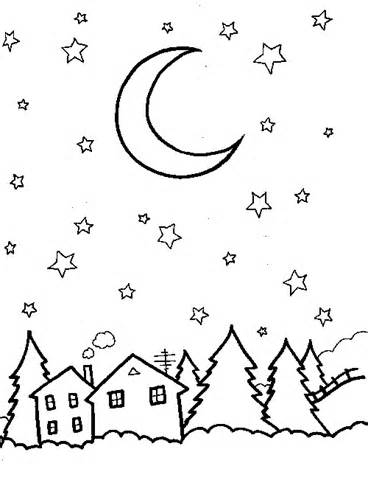
\includegraphics[width=0.4\textwidth]{ensavonds}
\end{intersong}
\beginsong{En 's Avonds}
\beginverse*
En 's avonds, en 's avonds, en 's avonds is het goed.
En 's avonds, en 's avonds, en 's avonds is het goed.
En 's avonds hebben we geld bij hopen,
en 's morgens geen om geld te kopen.
En 's avonds, en 's avonds, en 's avonds is het goed.
\endverse
\beginverse*
En 's avonds, en 's avonds, en 's avonds is het goed.
En 's avonds, en 's avonds, en 's avonds is het goed.
En 's avonds zouden we geerne trouwen,
en 's morgens nuchtens vroeg berouwen.
En 's avonds, en 's avonds, en 's avonds is het goed.
\endverse
\beginverse*
En 's avonds, en 's avonds, en 's avonds is het goed.
En 's avonds, en 's avonds, en 's avonds is het goed.
En 's avonds zullen wij koeken bakken,
en 's morgens tegen uw oren plakken.
En 's avonds, en 's avonds, en 's avonds is het goed.
\endverse
\endsong
\beginsong{En as ek komt te sterven}
\beginverse*
En as ek kom te stexwe,
Lief, sing dan g'n klaaglied nie
Plant dan g'n rose op my graf
Of koel sipresse nie.
Plant dan g'n rose op my graf
Of koel sipresse nie.
\endverse
\beginverse*
Laat net die groen gras bo mie wees
Die reen en die more dou.
En as jy wil vergeet my,
En as jy wil, onthou.
En as jy wil, vergeet mij,
En as jy wil, onthou.
\endverse
\beginverse*
Want skadu's sal'k nie sien,
Of voel hoe dat water week
Nie hoor hoe dat die voëltjies sing
As of hul harte breek.
Nie hoor hoe dat die voëltjies sing
As of hul harte breek.
\endverse
\beginverse*
Maar ek sal altyd drome dxoom
In die skemer; wie weet.
Miskien sal ek daar nog onthou,
Miskien sal ek vergeet.
Miskien sal ek daar nog onthou,
Miskien sal ek vergeet.
\endverse
\endsong
\beginsong{Mamma, 'k wil 'n man he!}
\beginverse*
Mamma, 'k wil 'n man he!
Watter man, m'n lieve kind,
Wil jy dan 'n Fransman he?
Nee, mamma, nee,
'n Franseman, die wil ek nie,
Want parlez-vous versta ek nie.
Dit is my plesier
Met die boerjongkerels hier.
\endverse
\beginverse*
Mamma, 'k wil 'n man he!
Watter man, m'n lieve kind,
Wil jy dan 'n Duitser he?
Nee, mamma, nee,
'n Duitseman, die wil ek nie,
Want schweinefleisch dat lus ek nie
Dit is my plesier
Met die boerjongkerels hier.
\endverse
\beginverse*
Mamma, 'kwil 'n manhe!
Watter man, m'n lieve kind,
Wil jy dan 'n boer soms he?
Ja, mamma, ja,
'n Boereman, die wil ek he,
In 'n boer syn arme wil ek le.
Dit is my plesier
Met die boerjongkerels hier
\endverse
\endsong
\beginsong{En revenant de Saint-Nazaire en France}
\beginverse*
En revenant de Saint-Nazaire en France
Oh lalalala - lalalala
En revenant de Saint-Nazaire en France
Tiens, voilà mon coeur
Tiens tiens tiens, voilà mon coeur.
\endverse
\beginverse*
J’ai rencontré trois belles filles Flamandes
J’en ai choisi la plus belle la plus grosse
Je l’ai donné un coup avec ma lance
Àprès trois mois, voilà le ventre qui gonfle
Àprès neuf mois, voilà le bébé qui chante
Àprès dix mois, elle veut que je recommence
Mais je n’avais plus de jus dans mes oranges. 
\endverse
\endsong
\begin{intersong}
    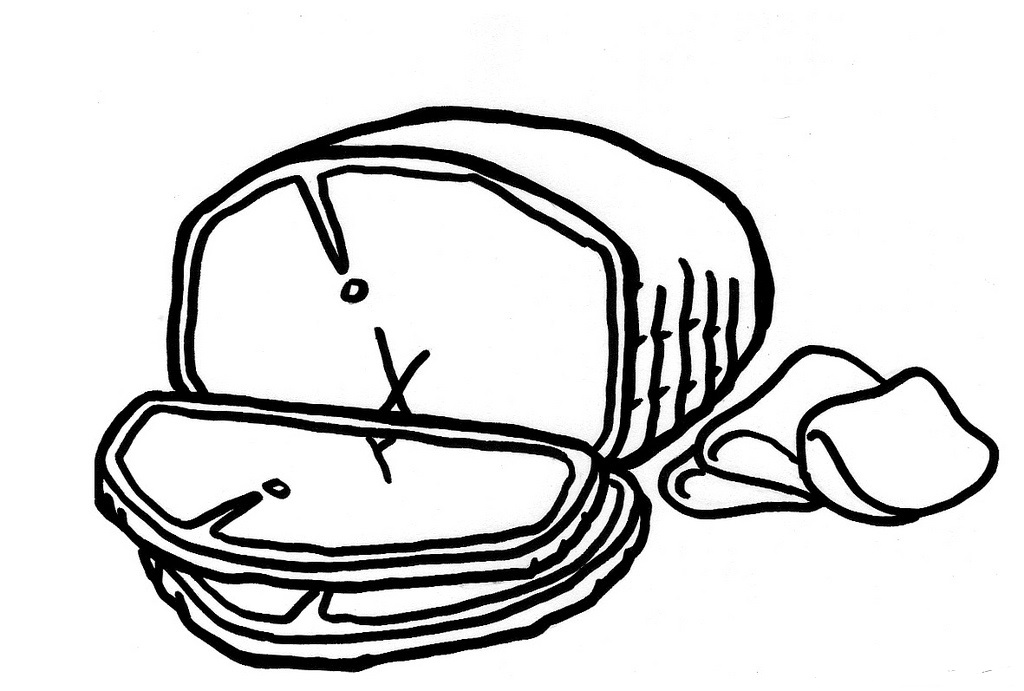
\includegraphics[width=0.4\textwidth]{ham}
\end{intersong}
\beginsong{Er is ham}
\beginverse
Er is ham, ham , voor op den boterham,
In de tent, in de tent, in de tent, in de tent,
Er is ham, ham, voor op den boterham,
In de fouragemeesters tent. 
\endverse
\beginchorus
Dat wist ik niet en bovendien, \rep{2}
Dat kon ik zonder bril niet zien   
\endchorus
\beginverse
Er is kaas, kaas, zo oud als sinterklaas.
\endverse
\beginverse
Er is soep, soep, voor een hongerige troep.
\endverse
\beginverse
Er is bier, bier, voor den aalmoezenier.
\endverse
\beginverse
Er is cake, cake, althans wat er op leek.
\endverse
\beginverse
Er is friet, friet, voor ieder een marmite. 
\endverse
\beginverse
Er is melk, melk, voor onze kleinste welp. 
\endverse
\beginverse
Er is cake, cake, vers van verleden week. 
\endverse
\endsong
\beginsong{Erika}
\beginverse*
Auf der Heide bluht ein kleines BIûmelein,
und das heißt, Erika.
Heiß von hunderttausend kleinen Bienelein,
wird umschwärmt, Erika.
Denn ihr Herz ist voller Sûssigkeit,
zarter duft entströmt dem BIûtekleid.
Auf der Heide blûht ein kleines Blûmelein,
und das heißt, Erika.
\endverse
\beginverse*
In der Heimat wohnt ein kleines Mägdelein,
und das heißt, Erika.
Dieses Mädel ist mein treues Schätzelein,
und mein Glûck, Erika.
Wenn das Heidekraut Rotlila blüht,
singe ich sum gruß ihr dieses Lied.
Auf der Heide blüht ein kleines …
\endverse
\endsong
\beginsong{Everywhere we go}
\beginchorus
Everywhere we go-o \rep{2}
People always ask us \rep{2}
Where do you come from \rep{2}
Where do you go to \rep{2}
And we shall always tell them \rep{2}	
We come from Nienof \rep{2}
Mary mary Nienof \rep{2}
And if they don’t hear us \rep{2}
We sing a little louder \rep{2}	
\endchorus
\beginchorus
They must be deaf!
\endchorus
\endsong
\beginsong{Geen regen kan ons deren}
\beginverse*
Geen regen kan ons deren, 
geen storm of geen geweld. 
Wanneer wij gaan marcheren, 
dan zijn wij rijk,
al hebben wij geen geld. 
Wij hebben slechts twee liefdes; 
Een voor het vlaamse land, 
en een ander voor Marieke, 
waarvoor mijn hartje brandt. 
Marie, Marie, Marie 'k zien a zeu geirn, 
ik blijf je trouw. Maar dienst is dienst, 
al doemet nie geirn. 
Wij zijn piot voor het vaderland, 
(stekt den boel in brand) 
marcheren wij, kreveren wij. 
Slechts na den dienst, 
falderie faldera, 
ben ik van jou en jij van mij, 
misschien, we zullen zien,...
\endverse
\endsong
\beginsong{Goede nacht, kameraden}
\beginverse*
Goede nacht, kameraden
Wij sluiten dezen dag
De sterren onzer lage landen,
Aan 't blauwe firmament,
Die zullen met hun glans de somberheid verbannen
\endverse
\endsong
\beginsong{Hand am Tich}
\beginverse
Hand am Tich, hand am tich, tra-lala-lalalala
Hand am Tich, hand am tich, tra-lala-lalalala.
\endverse
\beginverse
Zwei am Tich…
\endverse
\beginverse
Gatz von Stuhl…
\endverse
\beginverse
Fuz am Stuhl…
\endverse
\beginverse
Zwei am Stuhl…
\endverse
\beginverse
Tich von Grund…
\endverse
\beginverse
Hand von Tich…
\endverse
\beginverse
Hand am Glass…
\endverse
\beginverse
Trinken nur…
\endverse
\beginverse
EIN PROSIT…
\endverse
\beginverse
Glas am Tich…
\endverse
\beginverse
Hand von Glas…
\endverse
\beginverse
Hand am Tich…
\endverse
\beginverse
TIch am Grund…
\endverse
\beginverse
Fuz am Grund…
\endverse
\beginverse
Zwei am Grund…
\endverse
\beginverse
Hand von Tich…
\endverse
\beginverse
Zwei von Tich…
\endverse
\endsong
\beginsong{Heimwee doet ons hart verlangen}
\beginverse*
Heimwee doet ons hart verlangen,
naar de heimat onzer jeugd, naar de bronzen klokkenzangen,
zwaar van rouw of hel van vreugd.
Zangen uit de oude toren,
hij die waakt en verre schouwt,
over 't dorpje droomverloren,
kronk’lend aan zijn voet gebouwd.
\endverse
\beginverse*
Heimwee doet ons hart verlangen,
naar de geur van brem en hei,
naar de velden, mist omhangen,
op morgen in de mei.
Heimwee naar het blonde koren,
naar het dennebos vol peis.
Naar de vennen, stijf gevroren, 
waar wij slierden op het ijs.
\endverse
\beginverse*
Heimwee doet ons hart verlangen,
naar de ouderlijke haard.
Naar zijn rust niet te vervangen,
met zijn vrede welbewaard.
Heimwee naar de zomerwinden,
heimwee naar het zout geruis.
In de kruin der groene linden, 
voor ons oude pannenhuis
\endverse
\endsong
\begin{intersong}
    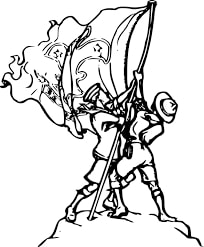
\includegraphics[width=0.4\textwidth]{hetvendel}
\end{intersong}
\beginsong{Het vendel}
\beginverse*
Het vendel moet marsjeren
want Vlaandren is in nood. 
Sint Joris geef ons kleren
geef ons soldij en brood. 
Dat wij geen koude lijden
Geef ons den boer zijn wijf
zijn wolhemd en zijn duiten
dat kan geen zonde zijn. 
\endverse
\beginchorus
Marsjeer, landsknecht marsjeer. 
\endchorus
\beginverse*
Wij slikken stof bij 't wandlen
verstomd zijn lied en lach. 
De keizer slikt heel Vlaandren
hij heeft een sterke maag(d).
Hij denkt al onder 't kauwen
Aan nieuwe roem en eer. 
Thuis weent een blonde vrouwe
als ik niet wederkeer. 
\endverse
\beginverse*
De tamboer slaat de parade
Sint Joris sterke held. 
Bescherm ons in genade
het vendel trekt te veld. 
De pijper wil niet fluiten
wij trekken stil en stom
over de groene heide
opwaarts naar Berg-op-zoom. 
\endverse
\endsong
\beginsong{Het zwartbruine bier}
\beginverse
Het zwartbruine bier, dat drink ik zo geern,
En zwartbruine meisjes, die kus ik zo geern.
Ei gij, ei gij, ei gij, bekoorlijk dudeldudeldij.
Juvivallerallera, juvivallerallera.
Ge laat geen rust aan mij.
\endverse
\beginverse
Het meisje heeft twee oogskens fijn,
Die fonk’len als een sterrekijn.
\endverse
\beginverse
Het meisje heeft een rozige mond,
En wie die kust die wordt gezond.
\endverse
\beginverse
Het meisje heeft een rozige kin,
Met in het midden een putteken erin.
\endverse
\beginverse
Het meisje heeft een hertekijn:
Dat zal wel voor eeuwig 't mijne zijn!
\endverse
\endsong
\beginsong{Hinky-Pinky}
\beginverse
En dit is de historie van een oude Chinees.
Hij heette Hinky-Pinky, da’s net zoveel als Kees.
Hij had een heel klein stalletje, aan de Chinese muur.
Hij verkocht er pinda’s, pinda’s, augurkjes in het zuur.
\endverse
\beginchorus
En van je hela hela hela ho lala
Hela hela hela ho lala
Hela hela hela ho lala
Hela hela ho lala
\endchorus
\beginverse
Hij verkocht ook bruine veters, maar die verkocht hij zwart
Per centi-centimeters, wat ging zijn zaakje hard.
De politie kwam eens kijken, hij moest uit China weg
Een kaartje voor de gevangenis, wat had die man een pech.
\endverse
\beginverse
En dit was dan d’historie, van een oude Chinees
Hij heette Hinky-Pinky, 't was net zoveel als Kees. 
\endverse
\endsong
\beginsong{Home on the range}
\beginverse
Oh give me a home,
where the buffalo roam,
where the deer and the antilope play.
Where the seldom is heard,
a discouraging word,
and the skies are not cloudy all day.
\endverse
\beginchorus
Home, home on the range,
where the deer and the antilope play.
Where seldom is heard
a discouraging word,
and the skies are not cloudy all day.
\endchorus
\beginverse
Oh, give me a land,
Where the bright diamond sand, 
Flows leisurely down the stream.
Where the graceful, white swan,
goes gliding along,
like a maid in a heavenly dream.
\endverse
\beginverse
Where the air is so pure,
the zephyrs so free,
the breezes so balmy and light.
That I would not exchange,
my home on the range,
for all of the cities so bright.
\endverse
\endsong
\beginsong{Hoog Op De Gele Wagen}
\beginverse*
Hoog op de gele wagen, rijd ik door berg en dal.
Lustig de kleppers draven, blij klinkt het hoorngeschal.
Waters en wouden en weiden, stromen zo machtig en vrij,
ik kan van uw schoon haast niet scheiden,
maar 't gaat voorbij en voorbij.
Ik kan van uw schoon haast niet scheiden,
maar 't gaat voorbij en voorbij.
\endverse
\endsong
\beginsong{Hoort gij ons dan niet roepen}
\beginverse
Hoort gij ons dan niet roepen,
de wolfjes die zijn hier. 
Sluit aan bij onze troepen,
kom jongens kom langs hier.
\endverse
\beginchorus
Wij doen ons best,
wij doen ons best,
wij doen ons bestebestebest.
Wij doen ons best
wij doen ons best
voor God en voor het Vlaamse land.
\endchorus
\beginverse
Al wat hier aan komt golven,
van Wolfjes, 't luistert al,
naar 't lied der Oude Wolven,
wij zwijgen overal.
\endverse
\beginverse
Het spelen moet ons sterken,
Maar eerlijk is ons spel!
En hoeven wij te werken,
dat doen wij even wel.
\endverse
\beginverse
Wij willen wolfjes blijven,
zolang wij zijn zo klein.
En willen 't zo ver drijven,
eens goede scouts te zijn.
\endverse
\endsong
\beginsong{If you’re happy and you know it}
\beginverse
if you’re happy and you know, it clap your hands
If you’re happy and you know, it clap your hands
If you’re happy and you know, it
And you really want to show, it
If you’re happy and you know, it clap your hands
\endverse
\beginchorus
Singing ja ja joepi joepi jee
Singing ja ja joepi joepi jee
Singing ja ja joepi, ja ja joepi,
Ja ja joepi joepi jee.
\endchorus
\beginverse
... stamp your feet…
\endverse
\beginverse
...say hey man…
\endverse
\beginverse
...give a kiss…
\endverse
\beginverse
...do all four…
\endverse
\endsong
\beginsong{De slag van Soetenaaie}
\beginverse*
Daar was ne keer de slag van Soetenaaie
Ge moest da zien, de slag der kurassier,
Kurassier, vooruit, geef vuur,
Met de linkerduim… 
\endverse
\beginchorus
Met de linkerduim; met de rechterduim;
Met de linkerhand; met de rechterhand;
Met de linkerarm; met de rechterarm;
Met het linkerbeen; met het rechterbeen; 
\endchorus
\endsong
\beginsong{Ik heb de zon zien zakken in de zee}
\beginverse
Ik heb de zon zien zakken in de zee.
Ik heb de zon zien zakken in de zee.
Ik heb de zon zien zakken, de zon zien zakken,
de zon zien zakken in de zee.
\endverse
\beginchorus
'k Zing van haja joepi, joepi, jee.
'k Zing van haja joepi, joepi, jee.
'k Zing van haja joepi, haja joepi,
haja joepi, joepi, jee.
\endchorus
\beginverse
Ik heb ze zon zien zeeen in de zak.
\endverse
\beginverse
Ik heb de zak zien zonnen in de zee.
\endverse
\beginverse
Ik heb de zak zien zeeen in de zon.
\endverse
\beginverse
Ik heb de zee zien zonnen in de zak.
\endverse
\beginverse
Ik heb de zee zien zakken in de zon.
\endverse
\endsong
\beginsong{Ik heb op zee mijn leven lang gevaren}
\beginverse*
Ik heb op zee, mijn leven lang gevaren,
mijn vissersdorp ligt aan het noordzeestrand.
Ik win mijn brood, met zwalpen op de baren,
toch denk ik vaak, mijn rijkdom ligt aan land.
\endverse
\beginchorus
Waar het lied der branding ruist bij dag en nacht,
waar 't vertrouwde huisje altijd op me wacht,
waar de meeuwen schreeuwen boven 't golfgedruis,
daar ben ik geboren, daar voel ik me thuis.
Waar de klokken luiden “visser vaar naar huis”
daar ben ik geboren, daar voel ik me thuis.
\endchorus
\beginverse*
Ik voel me klein, wanneer de stormen huilen,
bij donk’re nacht, belust op zwakke buit.
Maar voor geen geld ter wereld wil ik ruilen,
mijn vrij bestaan, als koning op mijn schuit.
\endverse
\endsong
\begin{intersong}
    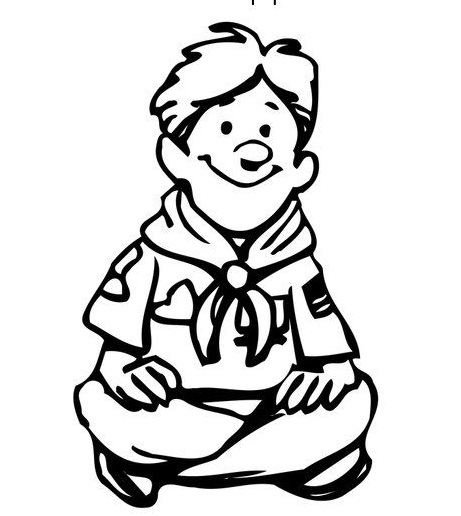
\includegraphics[width=0.4\textwidth]{inderonde}
\end{intersong}
\beginsong{In de ronde}
\beginverse*
Vrienden kom zit neder in de ronde
en genieten wij van deze stonde.
Al te samen, opgeruimd en blij
schuif wat dichter, dichter, dichter bij.
Al te samen, opgeruimd en blij
schuif wat dichter, dichter, dichter bij.
\endverse
\beginverse*
Denkt niet meer aan al die droeve dagen
met hun storm, wind en regenvlagen
Want de winter is al lang voorbij,
Al te samen, opgeruimd en blij
schuif wat dichter, dichter, dichter bij.
Al te samen, opgeruimd en blij
schuif wat dichter, dichter, dichter bij.
\endverse
\endsong
\beginsong{In De Stille Kempen}
\beginverse
In de stille Kempen op de purperen hei
Staat een eenzaam huisje met een berk erbij
Op een zomeravond in 't gedroom alleen
Kwam ik ongeweten langs dit huisje heen
\endverse
\beginchorus
Hoe schoon op de wereld
De zomerse hei
Dat is hier op aarde
De hemel voor mij
Hoe schoon nog de wereld
De zomerse hei
Dat is hier op aarde
De hemel voor mij
\endchorus
\beginverse
In dat eenzaam huisje zat een meisje, ach
Lijk ik nergens anders ooit een meisje zag
Door het venster keek ze mij verlegen aan
Schoof 't gordijntje toe en is maar opgestaan
\endverse
\beginverse
Maar wat heeft de liefde ook hier niet verricht
Want nu schuift 't gordijntje nooit meer voor mij dicht
Door het open venster dat men vroeger sloot
Lach ik op ons kindje op haar moeders schoot
\endverse
\beginverse
Dat is hier op aarde
De hemel voor mij
\endverse
\endsong
\beginsong{Op eer en trouw}
\beginverse*
Kom kameraden, kom
Kom kameraden, kom
Kom kameraden 
en meldt u blijde
Wij vinden paden in bos en hei.
\endverse
\beginverse*
Ons wachtwoord schalle
door heel de gouw
In dienst van allen
op eer en trouw.
\endverse
\beginverse*
Ons wachtwoord schalle
door heel de gouw
In dienst van allen
Op eer en trouw.
\endverse
\endsong
\beginsong{Van aan het frisse noordzeestrand}
\beginverse
Van  aan  het  frisse  noord – zee – strand
Tot  aan de  Kem – pische  hei
Daar  tre – kken  ke – rels  door  het  land
Zo  op - ge - wekt  e-en  blij  ( e-en blij)
\endverse
\beginchorus
Ha-ali hali halo, wij trekken 
wie trekt er met ons mee hali halo
Ha-ali hali halo wij trekken.
Wij zijn de Scouts, Hoezee !
\endchorus
\beginverse
Zo  tre – kken  wij  ons  le – ven  door
Steeds  op – ge – wekt  e-en  blij
En  vol – gen steeds  het  rechte  spoor
Dat  voert  ons  heme-elwaarts. (hemelwaarts)
\endverse
\endsong
\beginsong{In een klein stationnetje}
\beginverse*
In een klein stationnetje, 's morgen in de vroegte
Stonden zeven wagentjes, netjes op een rij
'k Zag een machinisteken, draaien aan een wieleken,
Hakke, hakke, tuut-tuut, weg zijn wij. 
\endverse
\beginverse*
In een klein stationnetje, laat al op de avond
Stonden zeven wagentjes, netjes op een rij
'k Zag een machinisteken, draaien aan een wieleken,
Hakke, hakke, tuut-tuut, weg zijn wij. 
\endverse
\beginverse*
In een klein stationnetje, laat al op de avond
Kwamen pa en ma gegaan, netjes op een rij
Ze namen 't machinisteken, vanachter 't klein wieleken. 
Nu maar gauw naar huis toe “do-do” doen. 
\endverse
\endsong
\beginsong{In het bos daar staat een huisje}
\beginverse*
In het bos daar staat een huisje
'k Keek eens door het vensterraam.
Er kwam een haasje aangelopen
't klopte even aan.
Help mij, help mij uit de nood,
of de jager schiet mij dood.
Laat mij in uw huisje klein,
'k Zal u dankbaar zijn. 
\endverse
\endsong
\beginsong{In München steht ein hofbräuhaus}
\beginverse*
Da wo die grüne Isar flüsst,
wo man mit Grüss Gott dich grüsst,
liegt meine schöne Münchnerstadt,
die ihres gleichen nicht had.
Wasser ist billig, frisch und gut,
nur verdünnt es unseres Blut.
Schöner sind tropfen goldnen weins,
aber am schönsten ist eins!
In München steht ein Hofbräuhaus,
eins, zwei, suffa.
Da läuft so manches Fässchen aus,
eins, zwei, suffa.
Da hat so mancher brave Mann,
eins, zwei, suffa,
gezigt was er schon vertragen kan.
Schon früh am Morgen fing er an,
und spät am Abend kam er nach Haus,
so schön ist’s im Hofbräuhaus!
Da trinkt man Bier nicht auf den Glas,
da gibt’s nur die grosse Hass,
und wen die erste Mass ist leer,
dan bringt dir die resl bald mehr.
Dann krigt zu Haus die Frau’nen schrek,
bleibt der Mann noch lange weg?
Aber die braven Nachbarleut,
die wissen besser bescheid!
\endverse
\endsong
\beginsong{In Seoul}
\beginverse*
In Seoul bij storm en bij regen,
Daar stond een vrijwilliger op wacht.
Hij hoorde de kreten der zege,
Maar plots trof een kogel hem in ’t hart.
En stervend zeeg hij, neder in die nacht,
Ja in die nacht
\endverse
\beginverse*
Gegroet mijn Vlaamse land,
Gegroet mijn meisje in ’t mooie Vlaamse land.
En stervend zeeg hij, neder in die nacht,
Ja in die nacht,
\endverse
\beginverse*
Gegroet mijn Vlaamse land,
Gegroet mijn meisje in ’t mooie Vlaamse land
\endverse
\endsong
\beginsong{Io Vivat}
\beginverse
Io vivat! io vivat!
Nostrarum sanitas!
Hoc est amoris poculum!
Doloris est antidotum!
\endverse
\beginverse
Io vivat! io vivat!
Nostrorum sanitas!
Dum nihil est in poculo,
Jam repleatur denuo!
\endverse
\beginverse
Io vivat! io vivat!
Nostrorum sanitas!
Nos jungit amicitia,
Et vinum praebet gaudia.
\endverse
\beginverse
Io vivat! io vivat!
Nostrorum sanitas!
Est vita nostra brevior,
et mors amara longior.
\endverse
\beginverse
Io vivat! io vivat!
Nostrorum sanitas!
Osores nostri pereant!
Amici semper floreant!
\endverse
\beginverse
Io vivat! io vivat!
Nostrorum sanitas!
Jam tota Academia ,
Nobiscum amet gaudia.
\endverse
\endsong
\beginsong{It's a long way}
\beginverse*
It’s a long way to Tipperary,
it’s a long way to go.
It’s a long way to Tipperary,
to the sweatest square I know.
Goodbye Piccadilly,
goodby Leicester square.
It’s a long way to Tipperary,
but my heart is still there.
\endverse
\endsong
\beginsong{Ja kamperen}
\beginverse
Ja kamperen is de mooiste zomersport
waardoor je steeds maar jonger wordt
je trekt door heel het mooie Vlaamse land
door bos en hei en strand.
\endverse
\beginchorus
Tralalalala, hey frieten met sala, hey
en een koude vla met nog een stukske
chocolalalal, hey frieten met sala, hey
en een koude vla met choclaaa…
\endchorus
\beginverse
De soep is soms een beetje aangebrand
dat vinden wij zo ambetant, 
de leiders zijn dan ook niet welgezind
en drinken gauw een pint.
\endverse
\beginverse
Het slapen gaat soms niet zo al te best
soms lig je in een mierennest,
je doet van heel de nacht geen oog meer dicht
tot aan het morgenlicht.
\endverse
\beginverse
En op de snelweg reed ne camion,
me aan het stuur een dikke non,
ze woog wel meer als honderdduuzend ton,
precies ne luchtballon.
\endverse
\endsong
\begin{intersong}
    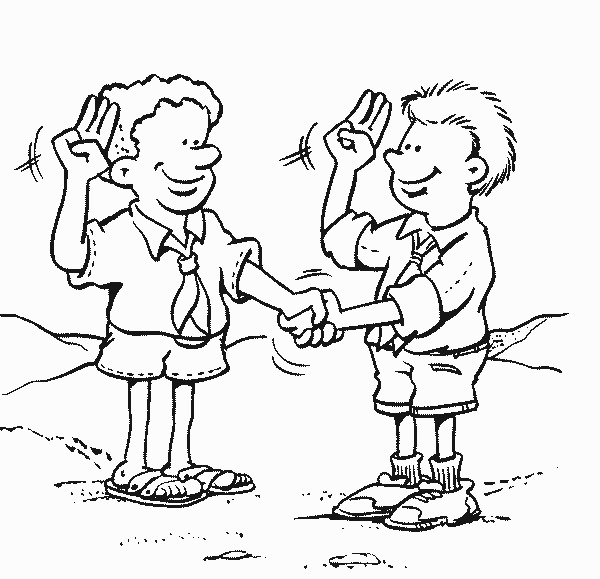
\includegraphics[width=0.4\textwidth]{janklaas}
\end{intersong}
\beginsong{Jan Klaas}
\beginverse
Jan Klaas wil wolfje worden,
din don deine, din don deine,
Jan Klaas wil wolfje worden,
maar hij weet niet hoe dat moet.
\endverse
\beginchorus
Dat is niet waar.

Beter is voor hem 
er maar niet bij te komen.
Beter is voor hem 
er maar niet bij te gaan.
\endchorus
\beginverse
Jan Klaas wil gaan kamperen,
maar hij weet niet waar naartoe
Zijn rugzak en zijn deken,
die zijn hem veel te zwaar.
\endverse
\endsong
\beginsong{Jef ge moetj nor oosj to goan}
\beginverse
Jef ge moetj nor oosj to goan a vraaken die es ziek \rep{2}
Es ze ziek, lotj ze ziek, stier ze mo nor de kliniek
en Jef ging nie nor oosj \rep{2}
\endverse
\beginchorus
Want, Jefken zijn leven was den boemlala, den boemlala, den boemlala, den boemla la
Jefken zijn leven was den boemlala, den boemlala. 
\endchorus
\beginverse
Jef ge moetj nor oosj to goan a vraaken die es deud	\rep{2}
Es ze deud, zee ma lank gekleut
en Jef ging nie nor oosj	\rep{2}
\endverse
\beginverse
Jef ge moetj nor oosj to goan a vraaken es in de kerk	\rep{2}
Es z’in de kerk, lotj z’in de kerk, tein ee meniër pastoer zij werk
en Jef ging nie nor oosj \rep{2}
\endverse
\beginverse
Jef ge moetj nor oosj to goan a vraaken es in’t graf \rep{2}
Es z’in 't graf, litj z’in 't graf, tein benne ker ver goe vanaf
en Jef ging nie nor oosj \rep{2}
\endverse
\beginverse
Jef ge moetj nor oosj to goan a vraaken es in d’hel	\rep{2}
Es z’in d’hel, lotj z’in d’hel, tein eet den duvel euk za spel
en Jef die ging nor oosj \rep{2}
\endverse
\endsong
\begin{intersong}
    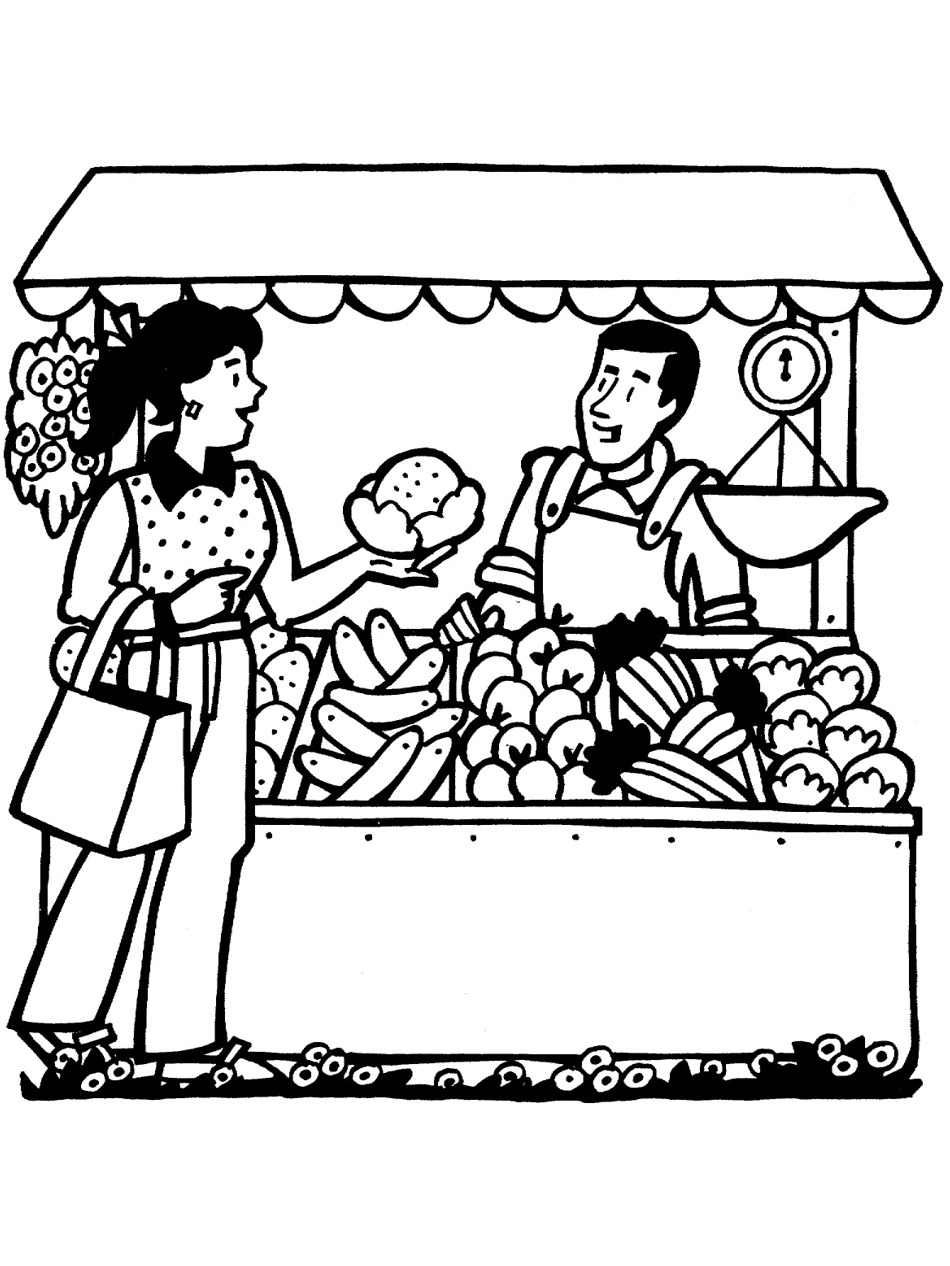
\includegraphics[width=0.4\textwidth]{jefzalveroonsgienkommissekesnimmerdoen}
\end{intersong}
\beginsong{Jef zal ver oons giën kommissekes nimmer doen}
\beginverse*
Jef zal ver ons giën kommissekes nimmer doen \rep{2}
Op zijn klein veloken \rep{2}
Jef zal ver ons giën kommissekes nimmer doen. 
\endverse
\endsong
\beginsong{JUCHHEIDI}
\beginverse
De student is een vrolijk nan,
Juchheidi, juchheida,
Zingt en drinkt zoveel hij kan,
Juchheidi, heida,
Springt en lacht maar altijd voort,
En kent nergens droevig oord.
\endverse
\beginchorus
Juchheidi, heidi, heida,
Juchheidi, juchheida,
Juchheidi, heidi, heida,
Juchheidi, heida.
\endchorus
\beginverse
Komt hij ene herberg in,
Hij drinkt immer blij van zin,
En is't met het geld gedaan,
Nog blijft zijne pret bestaan.
\endverse
\beginverse
Er blijft hem zo menig woon,
Waar men bier schenkt zonder loon,
En daarbij nog menig vriend
Die hem graag tot gastheer dient.
\endverse
\beginverse
Daarom zingt hij op de straat,
Blijde zangen vroeg en laat,
Minnend elke schone maagd
Oie hem naar zijn hartje zaagt.
\endverse
\beginverse
Munich, Hop, Jack-op of wijn,
't Kan hem nooit te vele zijn,
Altijd heeft hij honger, dorst,
wijl hij zingt uit volle borst.
\endverse
\beginverse
En zo leeft hij vrolijk voort,
In het schoon studentenoord,
Tussen boek en pijp en pint,
Waar elk meisje hem bemint.
\endverse
\beginverse
Overal de vlag in top!
Hel'dre ogen, warme kop.
En de strijdzang langs de ree:
"Vliegt de blauwvoet? Storm op Zee!”
\endverse
\beginverse
Leefden wij nog honderd jaar,
Nooit en rouwde 't onze schaar,
Al ons doen voor 't Vlaamse diet,
't Gildeleven, 't gildelied.
\endverse
\endsong
\beginsong{Kempenland}
\beginverse
Kempenland, aan de Dietse Kroon,
wonderfrisse parel;
Kempenland, welig zoete woon,
van de koene kerel;
\endverse
\beginchorus
Op de heide waait de wind
vrij van haag en heg
Op de heide waait de wind
alle zorgen weg.
\endchorus
\beginverse
Op de heide gloort de zon
ons zo stralend tegen.
Of uit frisse hemelbron,
ruist zo vree de regen.
\endverse
\beginverse
Op de heide staat een huis,
rondom in het lover.
Wolken blank als grauw of gruis
trekken traag daarover.
\endverse
\beginverse
Op de heide, zoete meid,
hebt ge mij verkoren.
Bij de gagel voor altijd,
mij uw trouw gezworen.
\endverse
\beginverse
Kempisch volk, zo vroom en blij
schoon van ziel en lijve.
Harde tijden gaan voorbij,
maar een volk moet blijven.
\endverse
\endsong
\beginsong{Kent gij Jan de mosselman}
\beginverse
Kent gij Jan de mosselman, de mosselman, de mosselman?
Kent gij Jan de mosselman, de man van Scheveningen?
\endverse
\beginverse*
Ja, ik ken de mosselman, de mosselman, de mosselman.
Ja, ik ken de mosselman, de man van Scheveningen.
\endverse
\beginverse*
Samen kennen wij de mosselman, de mosselman, de mosselman.
Samen kennen wij de mosselman, de man van Scheveningen.
\endverse
\endsong


\beginsong{Kijk dat eens aan}
\beginverse*
Kijk dat eens aan \rep{2}
Wat wilde troep \rep{2}
Wat hels lawaai \rep{2}
Wat dom geroep\rep{2}
\endverse
\beginchorus
Bij 't zien van zo’n kerels,
maakt U maar geen verdriet,
twee maanden bij de wolfjes,
en jij herkent ze niet.
\endchorus
\beginverse*
Ze lopen scheef \rep{2}
Ze staan niet fiks \rep{2}
Van rij of rang \rep{2}
Verstaan ze niets \rep{2}
\endverse
\beginverse*
Ze vinden niet \rep{2}
Een simpel spoor \rep{2}
langs pijl en kruis \rep{2}
Lopen ze door \rep{2}
\endverse
\beginverse*
Van fluit en mes \rep{2}
Van koord en staf \rep{2}
Weten ze niks \rep{2}
Volstrekt niks af \rep{2}
\endverse
\beginverse*
Ze weten niks \rep{2}
Van wet of groet \rep{2}
Van tweedeklas \rep{2}
Of tenderfoot \rep{2}
\endverse
\beginverse*
De knopen zijn \rep{2}
Hun onbekend \rep{2}
Ze kwamen nooit \rep{2}
In ene tent \rep{2}
\endverse
\beginverse*
Ze zijn zo dom \rep{2}
Zo vuil en wreed \rep{2}
En in een woord \rep{2}
Tot niks gereed \rep{2}
\endverse
\endsong
\beginsong{Klokke Roeland}
\beginverse*
Boven Gent rijst, eenzaam en grijs,
't Oud Belford, zinbeeld van 't verleden,
Somber en groots, steeds stom en doods,
Treurt d’ oude reus op 't Gent van heden,
Maar soms hij rilt en eensklaps gilt,
Zijn bronzen stemme door de stede.
Trilt in uw graf, trilt, Gentse helde,
Gij Jan Ryoens, Gij Artevelden,
Mijn naam is Roeland, 'k kleppe brand,
en luide storm in Vlaanderland.
\endverse
\beginverse*
En bont verschiet, Schept 't bronzen lied,
Prachtig weertov’rend mij voor d’ogen.
Mijn ziel herkent, Het oude Gent,
't volk komt gewapend toegevlogen:
't land is in nood “vrijheid of dood”,
De gilden komen aangetogen.
'k zie Jan Hyoens, 'k zie d’Artevelden,
en stormend roept Roeland de helden.
Mijn naam is Roeland, 'k kleppe brand,
En luide storm in Vlaanderland.
\endverse
\beginverse*
O heldentolk, O reuzenvolk,
O pracht en macht van vroeger dagen,
O bronzen lied, 'k Wete uw bedied,
En ik versta 't verwijtend klagen,
Doch wees getroost: zie 't Oosten bloost,
En vlaanderens zonne gaat aan 't dagen
“Vlaanderen die leu”, tril, oude toren,
En paar een lied met onze koren;
Zing “Ik ben Roeland, 'k kleppe brand,
Luide triomf in Vlaanderenland!”.
\endverse
\endsong
\beginsong{Kom maar aan je deuren kijken}
\beginverse*
Kom maar aan je deuren kijken,
open uwe ramen wijd.
Want hier zijn de vlaamse trekkers,
trekkers van de nieuwe tijd.
Waar wij blijde mensen groeten,
klinkt ons staplied dubbel hard.
Zien wij soms droeve gezichten,
dan schenkt ons eerder vreugd’ dan smart.
Zingend Vlaand’ren trouw te dienen,
faja faja faja faja hop hop hop.
met ons doel valt niet te grienen,
Faja faja faja faja hop hop hop

\endverse
\endsong
\begin{intersong}
    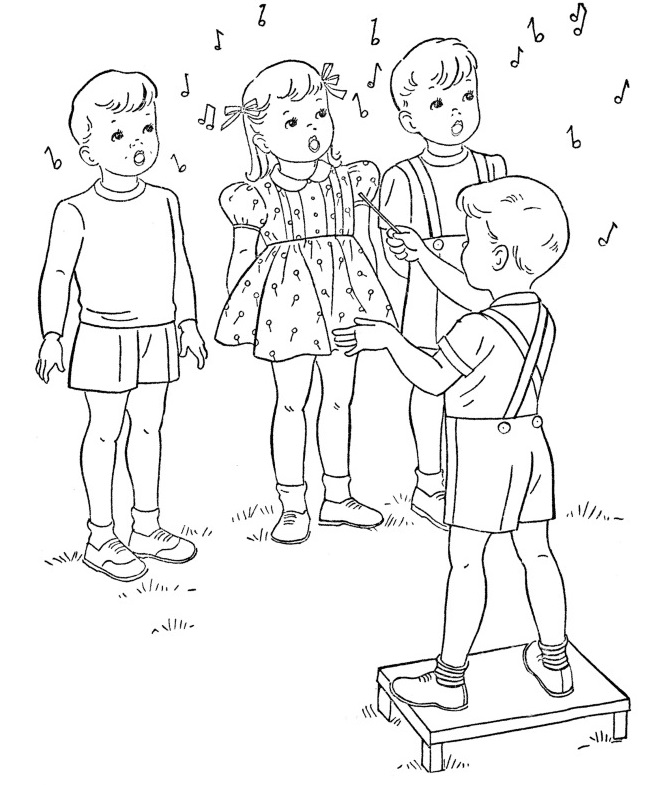
\includegraphics[width=0.4\textwidth]{kumbayamylord}
\end{intersong}
\beginsong{Kumbaya my lord}
\beginverse*
Kumbaya my lord, kumbaya \rep{3}
Oh, lord, kumbaya \rep{2}
\endverse
\beginchorus
-	Someone’s singing my lord, kumbaya \rep{3}
-	Someone’s sleeping my lord, kumbaya	\rep{3}
-	Someon’s praying my lord, kumbaya	\rep{3}

\endchorus
\endsong 
\beginsong{Laat ons een bloem}
\beginverse
Dit is een lied voor de mensen die zorgen,
dat morgen de mensen al dood zullen zijn.
Dit is een lied voor de doden van morgen,
begraven, bekist in een stenen woestijn. 
\endverse
\beginchorus
Laat ons een bloem en wat gras dat nog groen is
Laat ons een boom en het zicht op de zee.
Vergeet voor een keer hoeveel geld een miljoen is
De wereld, die moet nog een eeuwigheid mee. 
\endchorus
\beginverse
Je breekt en je hakt en je boort door de bergen,
je maakt elke heuvel gelijk met de grond.
De reuzen van nu lijken morgen maar dwergen
vooruitgang vernieuwt wat er gisteren nog stond. 
\endverse
\beginverse
De vis in de zeeën vergiftigd gestorven,
Het zand op het strand vervuild met mazout. 
En jij door de tankers en chequeboek bedorven,
Je weet zelf niet meer waar de meeuw heeft gebroed. 
\endverse
\beginverse
En zo zal dan morgen het leven verdwijnen,
verslagen door staal en gewapend beton.
De maan zal dan koud op je nachtmerrie schijnen
geen mens die nog weet hoe 't einde begon. 
\endverse
\endsong
\beginsong{Les Montagnards}
\beginverse
Montagnes Pyrénées, je t’aimerai toujours.
Montagnes fortunées, je t’aimerai toujours.
Rien n’est si beau que mon pays, que mon pays.
Rien n’est si beau que ma patrie, que ma patrie. 
Les Montagnards, les Montagnards,
Chantez en coeur, chantez en coeur,
De mon pays, de mon pays, 
La joie. Et le bonheur, et le bonheur.
La la lala lala la la lala la la
\endverse
\beginchorus
Altla altla altla: les Montagnards, les Montagnards,
Altla altla altla: les Montagnards sont là.
Les Montagnards, les Montagnards sont là.
\endchorus
\endsong
\beginsong{Let it be}
\beginverse
When I find myself in times of trouble
Mother Mary comes to me,
Speaking words of wisdom: let it be. 
And in my hour of darknes,
She is standing right in front of me,
Speaking words of wisdom: let it be. 
\endverse
\beginchorus
1:
Let it be, let it be, let it be, let it be
Whisper words of wisdom: let it be.

2:
Let it be, let it be, let it be, let it be
Yeh, there will be an answer: let it be
\endchorus
\beginverse*
And when the broken-hearted people
Living in the world  agree,
There will be an answer: let it be.
For tho’they may be parted,
There is still a chance that they will see,
There will be an answer, let it be. 
\endverse
\beginverse*
And when the night is cloudy,
There is still a light that shines on me
Shine until tomorrow, let it be. 
I wake up to the sound of music, 
Mother Mary comes to me,
Speaking words of wisdom: let it be. 
\endverse
\endsong
\beginsong{Lili-Marleen}
\beginverse*
Vor der Kaserne, vor dem grossen Tor,
stand eine Lanterne und steht sie noch davor.
So wollen wir un wiedersehn,
bei der Lanterne woll’n wir stehn.
Wie einst Lili-Marleen.
\endverse
\endsong
\beginsong{Loch Lomon}
\beginverse*
By you bonnie banks and by yon bonnie braes,
Where the sun shines bright on Loch Lomon’
Where we and my true love were ever wont to be
On the bonnie, bonnie banks of Loch Lomon’
\endverse
\beginchorus
Oh you’ll take the high road, and I’ll take the low road,
And I’ll be in Scotland before you,
But me and my true love will never meet again,
On the bonnie, bonnie banks of Loch Lomon’.
\endchorus
\beginverse*
I mind where we parted in yon shady glen,
On the steep, steep side of Ben Lomon’
Where in deep purple hue, the Highlands hills we view
And the moon coming out in the gloaming. 
The wee birdies sing and the wild flowers spring
And in sunshine the waters are sleeping;
But the broken heart will ken no second spring again,
And the world does not know how we are greating. 
\endverse
\beginverse*
En ik em er goed af, mo gau zetj er slecht van
En gau gotj go sloapen, nog veer mau
Want ik em ervoaring en gau, gau zetj just niks
On the bonnie bonnie banks of the bartentj.
\endverse
\endsong
\beginsong{Marmelade}
\beginverse*
Marmelade, karbonade, varkenspootjes, bloemkool en salade.
O koekjeskruimels, o slagroomtaartjes,
Lange vingers, pannenkoeken,
\endverse
\beginchorus
Honger
Honger
Honger
Honger
Honger
\endchorus
\endsong
\beginsong{Met de trouwe totempaal vooraan}
\beginverse*
Met de trouwe totempaal vooraan,
Stapt de horde zingend langs de baan,
En met gulle lach om monden blij,
Stappen welpen netjes in de rij. 
Links, rechts, links, en voet na voet
Vooruit marsjeren maakt ons niet zo moe.
Links, rechts, links en stap na stap,
We trekken zingend naar de djungle toe. 
\endverse
\endsong
\beginsong{Met mijn hand op mezelf}
\beginverse*
Met mijn hand op mezelf, en wat heb ik daar?
Dat is mijn leerkastje zeg ik voorwaar.
Leerkastje… hollebolle krullekop
Dat is 't geen ik leerde bij meester Top.
\endverse
\beginchorus
--Iedere strofe een woord bijvoegen--
leerkijkers, snotneusje, notenkrakers,
kinneborstei, langnekje,
broodmandje, knieknikkers, 
kaasdoosjes.
\endchorus
\endsong
\beginsong{Mijn hoed die heeft vier deuken}
\beginverse*
Mijn hoed die heeft vier deuken.
Vier deuken heeft mijn hoed.
En had mijn hoed geen vier deuken.
Dan was hij mijn hoed niet meer.
\endverse
\endsong
\beginsong{Mijn vader is bakker}
\beginverse
Mijn vader is bakker, zijn zoontje ben ik,
Mijn vader bakt broodjes, ze eten doe ik.
\endverse
\beginchorus
Holadi-jee, holadi-jo
Holad-jopsasa, holadi-jee 
\rep{2}
\endchorus
\beginverse
Mijn vader is metser, zijn zoontje ben ik,
Mijn vader metst muurtjes, daartegen plas ik.
\endverse
\beginverse
Mijn vader is brouwer, zijn zoontje ben ik,
Mijn vader brouwt biertjes, ze drinken doe ik. 
\endverse
\beginverse
Mijn vader is brandweer, zijn zoontje ben ik, 
Mijn vader blust brandjes, ze stichten doe ik.
\endverse
\beginverse
Mijn vader is dominee, zijn zoontje ben ik,
Mijn vader huwt meisjes, ze kussen doe ik. 
\endverse
\endsong
\beginsong{Mijne vlieger}
\beginverse*
'k Ben nie al te zot van 't spel, mor 'k vange gere musschen. 
Marblen en toppen kan ik wel, daarin ben ik nie fel.
'k Zie tegenwoordig overal, en ook al in mijn straatje,
Jongens schuppen op nen bal, mo 'k spele 't liefst van al
\endverse
\beginchorus
Mee mijnen vlieger, en zijne steert,
Hij goot omhuuge, 't es 't ziene weert,
'k geve mor klauwe, op mijn gemak,
'k hem nog drei bollekes, in mijnen zak. 
\endchorus
\beginverse*
Mietje van de koolmarchang, een meisken uit mijn strotjen,
Keurde mijne cervolant, en z’had er 't handje van,
Want zo rap als de wind was z’aan 't spelen met mijn klauwe,
En ze riep 't es 't spelen weert, want hij ee ne goeie steert. 
Ja mijne vlieger … twee bollekes … 
\endverse
\beginverse*
't Seef liet zijne vlieger op van 't soepe, 't soepe, 't soepe,
Maar hij stuikt op zijne kop, en muile dat hij trok. 
Zij spankoorde was veel te kort, en met zijn 't sietse klauwe, 
En daarbij was zijne steert gen chique toebak weert.
Maar mijne vlieger … één bolleken …
\endverse
\beginverse*
Laatst op 't Sint-Denijsplein, mijne vlieger was aan’t zweve,
d’er kwam een wijf, een groot venijn, ze zei dat mag niet zijn. 
Hij hangt te veel in mijne weg, en ze begost er aan te sleuren,
En op een twee drei pardaf, de koorde schoot er af…
\endverse
\beginchorus
Hij was go vliegen, al mee de wind,
'k Stonde te schrieme, 'k was mor e kind,
Mijnen bol klauwe, die ging ne gang,
Dat zal 'k omtauwe, mijn leven lang…  
\endchorus
\endsong 
\beginsong{My Bonnie is over the ocean}
\beginverse*
My Bonnie is over the ocean.
My Bonnie is over the sea.
My Bonnie is over the ocean.
O bring back my Bonnie to me.
\endverse
\beginchorus
Bring back, bring back
Bring back my Bonnie to me, to me
Bring back, bring back
O bring back my Bonnie to me.
\endchorus
\beginverse*
Last night as I lay on my pillow,
Last night as I lay on my bed,
Last night as I lay on my pillow,
I dreamed that my Bonnie was dead.
\endverse
\beginverse*
The winds have blown over the ocean,
The winds have blown over the sea,
The winds have blown over the ocean,
And brought back my Bonnie to me.
\endverse
\beginverse*
Man bommau marsjeert op gallosjen,
man bommau marsjeert in de sjnieè,
man  bommau marsjeert op gallosjen,
en zee gien kou voeten ne mie.
\endverse
\beginverse*
Man bompa die drinkt altijd vaarzen,
man bompa die is altijd zat, 
man bompa die drinkt altijd vaarzen,
en s’anderdaags leit em weer plat!
\endverse
\endsong 
\beginsong{Nobody Knows}
\beginverse*
Nobody knows, the trouble I’ve seen,
nobody knows, but Jesus,
nobody knows, the trouble I’ve seen,
glory, hallelujah
\endverse
\beginverse*
Sometimes I’m up, sometimes I’m down,
oh yes, lord.
Sometimes I’m almost to the ground,
oh yes, Lord.
\endverse
\beginverse*
Oh everyday to you I pray,
oh yes, Lord.
For you to drive my sins away, 
oh yes, Lord.
If you get there before I do,
oh yes, Lord
Tell all my friends I’m coming too,
oh yes, Lord.
\endverse
\endsong
\beginsong{Nooi van die velde}
\beginverse*
O nooi van die velde wat is jy tog skoon
ek het jou in stede nog nimmer sien woon,
maar ver op die velde waar son altyd skyn
is mooier die nooitjies en beter die wyn. 
Tralalalalala
\endverse
\beginverse*
O nooi van die velde wat is jij tog mooi
met vange wat gloei van die more se rooi,
daar verop die velde waar son altyd skyn,
is rooier die lippies en rooier die wyn.
Tralalalalala
\endverse
\beginverse*
O nooi van die velde jou kus en jou lag
soos water wat kabbel oor klippies so sag
daar ver op die velde waar son altyd skyn
is soeter die soentjies en soeter die wyn
Tralalalalala
\endverse
\endsong
\beginsong{O mijn Kempen}
\beginverse*
Geen land ook ter wereld, hoe schoon of hoe rijk,
Is 't land van mijn harte, mijn heimat gelijk.
Hier zaaiden ons handen en groeit er ons brood.
Hier vinden wie gingen de rust in de dood.
Hier stap'len de wolken kastelen opeen,
En giert er een Noorzee heur wind om ons heen!
Hier jubelt de zomer in heide en ven:
Hoe heerlijk de Kempen, zo schoon ik niets ken!
\endverse
\beginchorus
0 mijn Kempen, ja mijn Kempen!
0 mijn enig heimatland.
En waarvoor een vlam van liefde
Eeuwig in mijn harte brandt!
\endchorus
\beginverse*
Hier malen de molens de rust over 't land,
Verdolen de wegels in't stuivende zand.
Hier heersen de vlakten en ruiselt ons lied,
Beklemmen geen verten het vrije verschiet.
Het goud van uw zandzee, het purper der hei
Het tovert visioenen van wellust in mij.
Van dennen en berken, van berken en den,
Hoe heerlijk de Kempen, zo schoon ik niets ken!
\endverse
\endsong 
\beginsong{O when the saints}
\beginverse*
O when the saints, o when the saints,
go marchin in, go marchin in,
O when the saints go marching in.
I want to be in that number.
O when the saints go marching in.
\endverse
\beginchorus
I’ve got in love a father,
he’s gone to heaven I know.
But I would meet him,
when the saints go marching in.
\endchorus
\endsong 
\beginsong{O’ Pescator}
\beginverse*
O pescator dell’ ondé
O Frederi
Vieni a pescar in qua
Sulla tua bella barca
La pui bella se ne va
Frederi -la -la
\rep{2}
\endverse
\beginverse*
Che casa vuol oh’io peschi	
O Frederi			
L’avel che un’e casca		
Sulla tua…			
\rep{2}
\endverse
\beginverse*
Ti daro cento scudi	
O Frederi		
Sta borsa ricanna	
Sulla...			
\rep{2}
\endverse
\beginverse*
Non voglio cento sendi	
O Frederi		
Ne borsa ricanna	
Sulla…			
\rep{2}
\endverse
\endsong
\beginsong{Ochtendlied}
\beginverse*
Broers haal op de dag begint te rijzen,
de vlag gehesen naar de zon. 
Ziet de gouden spies ten hemel wijzen,
de dag die weer begon. 
Laat uw licht weerstralen in de harten, 
laat uw licht het grauwe duister tarten. 
Broers gedraag u fris door heel de dag,
de gave van onze lach. 
Brand de reinheid van Gods dageraad,
in 't adel van uw gelaat. 
\endverse
\endsong
\begin{intersong}
    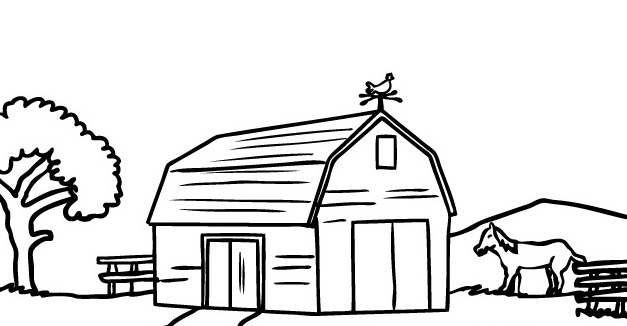
\includegraphics[width=0.4\textwidth]{oldmacdonald}
\end{intersong}
\beginsong{Old Mac Donald}
\beginverse*
Old Mac Donald had a farm, e-i-e-i-o,
and on farm he had some chicks, e-i-e-i-o
with a chick-chick here and a chick-chick there,
here chick, there chick,
everywhere a chick-chick,
old Mac Donald had a farm, e-i-e-i-o
\endverse
\beginverse*
… some ducks - quack-quack
… some cows - moo-moo
… some pigs - oink-oink
… some cats - mauw-mauw
… some dogs - wouf-wouf
… a car - broom-broom
\endverse
\endsong 
\beginsong{Omer Gaspard}
\beginverse*
Allons, Omer Gaspard,
encore un verre,
encore un verre, encore
Allons Omer Gaspard,
encore un verre,
et ça fait tard.
\endverse
\beginverse*
Si paternel,
si paternel revient,
on lui dira
son verre est toujours,
plein, plein, plein,…
\endverse
\endsong 
\beginsong{Ons devies is dienen}
\beginverse*
Ons devies is dienen, Ridders van de Daad,
Ons devies is dienen, Ridders van de Daad.
Want padvinders marcheren, door heel 't Vlaanderland,
Want padvinders marcheren, door heel 't Vlaanderland.
Geel, groen, rood zijn kleuren, van ons broederschap,
Geel, groen, rood zijn kleuren, van ons broederschap.
Want padvinders marcheren, door heel 't Vlaanderland,
Want padvinders marcheren, door heel 't Vlaanderland.
\endverse
\endsong 
\beginsong{Ontwaakt gij luie slapers}
\beginverse*
Ontwaakt gij luie slapers
De koekoek roept U op.
\endverse
\beginverse*
Wordt wakker, wordt wakker
De koekoek roept U op. \rep{2}
\endverse
\beginverse*
Koekoek, koekoek,
De koekoek roept U op. \rep{2}
\endverse
\beginverse*
De zon kleurt met haar stralen
Den groenen heuveltop.
\endverse
\endsong 
\beginsong{Patrouilleleiders komen getreden}
\beginverse*
Patrouilleleiders komen getreden,
Verbonden door eenzelfde wet,
Zij willen een spoorteken wezen,
Een spoor dat de anderen redt,
Zij willen een spoorteken wezen,
Een spoor dat de anderen redt.
\endverse
\beginverse*
En daarom reik mij je hand, kameraden,
Zo gaan wij tesamen vooraan,
Dan mag ons de wereld verraden,
Onz’ vriendschap blijft eeuwig bestaan,
Dan mag ons de wereld verraden,
Onz’ vriendschap blijft eeuwig bestaan,
\endverse
\beginverse*
Wij hebben ons woord eens gegeven, 
Ach woorden vergaan soms zo vlug,
De andren zij mogen begeven,
Doch wij willen niet meer terug,
De andren zij mogen begeven,
Doch wij willen niet meer terug.
\endverse
\endsong 
\beginsong{Rij maar an … ossewä}
\beginverse*
Rij maar an, ossewä, rij maar an… \rep{2}
Weet je wel waarheen ie ga?
Wel naar huis toe rij die wä.
Rij maar an, ossewä, rij maar an.
\endverse
\beginverse*
Zachtjes naar het maïsveld. \rep{2}
Daar lä men die ossewä.
En weldra is ie kant en klaar.
\endverse
\beginverse*
Zachtjes trekke, niet te snel,
anders wordt die os te moe…
Langsam an en niet te snel,
bereiken zal j’ons huisje wel.
\endverse
\endsong 
\beginsong{Roosmarijntje}
\beginverse*
Roosmarijntje: rozenmond!
Wist je mijn verlangen!
Roosmarijntje: rozenmond
met je bolle wangen.
\endverse
\beginchorus
Links en rechts moet ik marcheren,
Links en rechts aan u voorbij;
Tussen helmen en geweren,
Schoon ik met u vrij.
\endchorus
\beginverse*
Roosmarijntje: blonde kind
Met je blauwe ogen,
Met je haren in de wind,
Nooit heb 'k u belogen!
\endverse
\beginverse*
Roosmarijntje: kleine vrouw
Met je vele zorgen,
Als ik morgen met je trouw
Ligt een schat geborgen!
\endverse
\beginverse*
Roosmarijntje: schattebout;
Heerlijk moet het wezen,
Als g’ ons eerste kindje douwt
Uit een droom gerezen. 
\endverse
\endsong
\beginsong{Sarie Marais}
\beginverse*
Mij Sarie Marais is so ver van mij hart
maar 'k hoop om haar weer te sien.
Sij het in die wijk van die mooirivier gewoon,
nog voor die oorlog het begin.
\endverse
\beginchorus
O bring mij trug na die ou transvaal,
daar waar mijn Sarie woon.
Daar onder in die mielies bij die groen doringboom,
daar woon mij Sarie Marais.
Daar onder in die mielies bij die groen doringboom,
daar woon mij Sarie Marais.
\endchorus
\beginverse*
Ek was so bang dat die kakies mij sou vang,
en ver oor die see wegstuur.
Toe vlug ek na die kant van die Upinhton se sand,
daar onder langs die grootrivier.
\endverse
\beginverse*
Die kakies is mos net soos’n krokodillepes,
hul sleep jou altijd watertoe.
Hul gooi op’n skip vir’n lange lange trip,
die josie weet waar na toe.
\endverse
\beginverse*
Verlossing het gekom, en die huistoe gaan was daar,
trug na die ou transvaal.
Mij lievelingspersoon sal seker ook daar wees,
om mij met 'n kus te beloon.
\endverse
\endsong
\beginsong{Schoon klaart de dag}
\beginverse*
Schoon klaart de dag, hoog waait de vlag,
Wie niet dapper is kan bij ons niets staan,
Wie niet durven kan moet ten onder gaan,
Komt straks de harde strijd, wij zijn bereid.
\endverse
\beginverse*
Eens komt het uur, gloeiend als vuur,
Dat de vijand grimmig voor ons staat,
En het uur der Vlaamse zege slaat,
Komt straks de harde strijd, wij zijn bereid.
\endverse
\beginverse*
Trouw tot de dood, Vlaanderen wordt groot,
Als gij morgen valt en ik blijf alleen,
Kameraad, 'k blijf trouw en ik vecht voor twee.
Komt straks de harde strijd, wij zijn bereid.
\endverse
\endsong
\beginsong{'t Ros Beyaard}
\beginverse*
't Ros Beyaard doet zijn ronde 
In de stad van Dendermonde; 
Die van Aalst die zijn zo kwaad
Omdat hier 't Ros Beyaard gaat. 
\endverse
\beginverse*
De vier Aymonskinderen jent 
met blanke zweerd in d'hand 
Ziet ze rijden: 't zijn de
schoonste al van ons land! 
\endverse
\beginverse*
t'Ros Beyaarrts ogen fonklen,
Zijne brede manen kronklen,
En hij wendt hem fraai en vlug,
Met vier broers op zijnen rug.
\endverse
\beginverse*
't Ros Beyaard is verheven,
Heeft hem in het vuur begeven,
En week op 't oorlogsveld,
Alles voor zijn groot geweld.
\endverse
\endsong
\beginsong{Taptoelied}
\beginverse*
'd Avond valt, alles zwijgt
Zachtjes ruist over zee, bos en hei
Winden groet, alles goed
God nabij. 
\endverse
\endsong
\beginsong{Taraboemdery}
\beginverse*
Eitemal – 'n Sweedse volkswysie
\endverse
\beginverse*
Taraboemdery, my va-aal haar noointjie
Taraboemdery, o wees nie bang nie
Nee, o nee, o nee, dis nie-ie meer lank nie
Dan is e-ek weer a-aan jou sy.
\endverse
\beginchorus
Taraboemdery-y, ra-boemdery, boemdery
Taraboemdery-y, ra-boemdery, boem, boem, boem.
\endchorus
\beginverse*
Taraboemdery, my va-aal haar noointjie
Taraboemdery, hoe brand die wonde !
Wee, o wee, o wee, van da-aar die stonde
Toe ons ho-oor, dat o-ons moe skei.
\endverse
\beginverse*
Taraboemdery, my va-aal haar noointjie
Taraboemdery, die lange nagte
Lang, o lang,o lang, aanho-oor my klagte
Stil van sto-omme me-edely.
\endverse
\beginverse*
Taraboemdery, my va-aal haar noointjie
Taraboemdery, verwag my more
Blye, blanke dag, as o-oggendglore
Oor jou blo-onde ha-are gly.
\endverse
\endsong 
\beginsong{There was a devil woman}
\beginverse*
There was a devil woman, 
and she lived in the wood,
waila waila woula.
There was a devil woman,
and she lived in the wood,
down by the river Sawayer.
\endverse
\beginverse*
She had a baby three months old.
\endverse
\beginverse*
She had a pen knife long and sharp.
\endverse
\beginverse*
She stook the knife in the babys head.
\endverse
\beginverse*
There were three bond knocks from a knocking on the door.
\endverse
\beginverse*
There were two policemen and a special-branch man.
\endverse
\beginverse*
Are you the woman who killed that child.
\endverse
\beginverse*
They took her away and put her in the jail.
\endverse
\beginverse*
They put a rope around her neck.
\endverse
\beginverse*
They pulled the rope and she got hung.
\endverse
\beginverse*
So that was the end,
of the woman in the wood,
waila waila woula.
So that was the end,
of the baby too,
down by the river Sawayer.
\endverse
\endsong
\beginsong{Tien kleine negers}
\beginverse*
Tien kleine negers,
die speelden in de regen,
eentje werd er doodgeregend,
toen waren ze nog met negen.
\endverse
\beginverse*
Negen kleine negers,
die speelden in de gracht,
eentje werd er doodgegracht,
toen waren ze nog met acht.
\endverse
\beginverse*
Acht kleine negers,
die stonden daar te beven,
eentje werd er doodgebeefd,
toen waren ze nog met zeven.
\endverse
\beginverse*
Zeven kleine negers,
die speelden met een mes,
eentje werd er doodgemest,
toen waren ze nog met zes.
\endverse
\beginverse*
Zes kleine negers,
die speelden met een Zeis,
eentje werd er doodgezeist,
toen waren ze nog met vijf.
\endverse
\beginverse*
Vijf kleine negers,
die speelden met een pier,
eentje werd er doodgepierd,
toen waren ze nog met vier.
\endverse
\beginverse*
Vier kleine negers,
die speelden met een spie,
eentje werd er doodgespied,
toen waren ze nog met drie.
\endverse
\beginverse*
Drie kleine negers,
die speelden op een tree,
eentje werd er doodgetreed,
toen waren ze nog met twee.
\endverse
\beginverse*
Twee kleine negers,
die speelden met een been,
eentje werd er doodgebeend,
toen was er nog maar een.
\endverse
\beginverse*
Een kleine neger,
die speelde met Marie,
ze kregen vele kind'ren,
en nu zijn ze weer met tien.
\endverse
\endsong
\begin{intersong}
    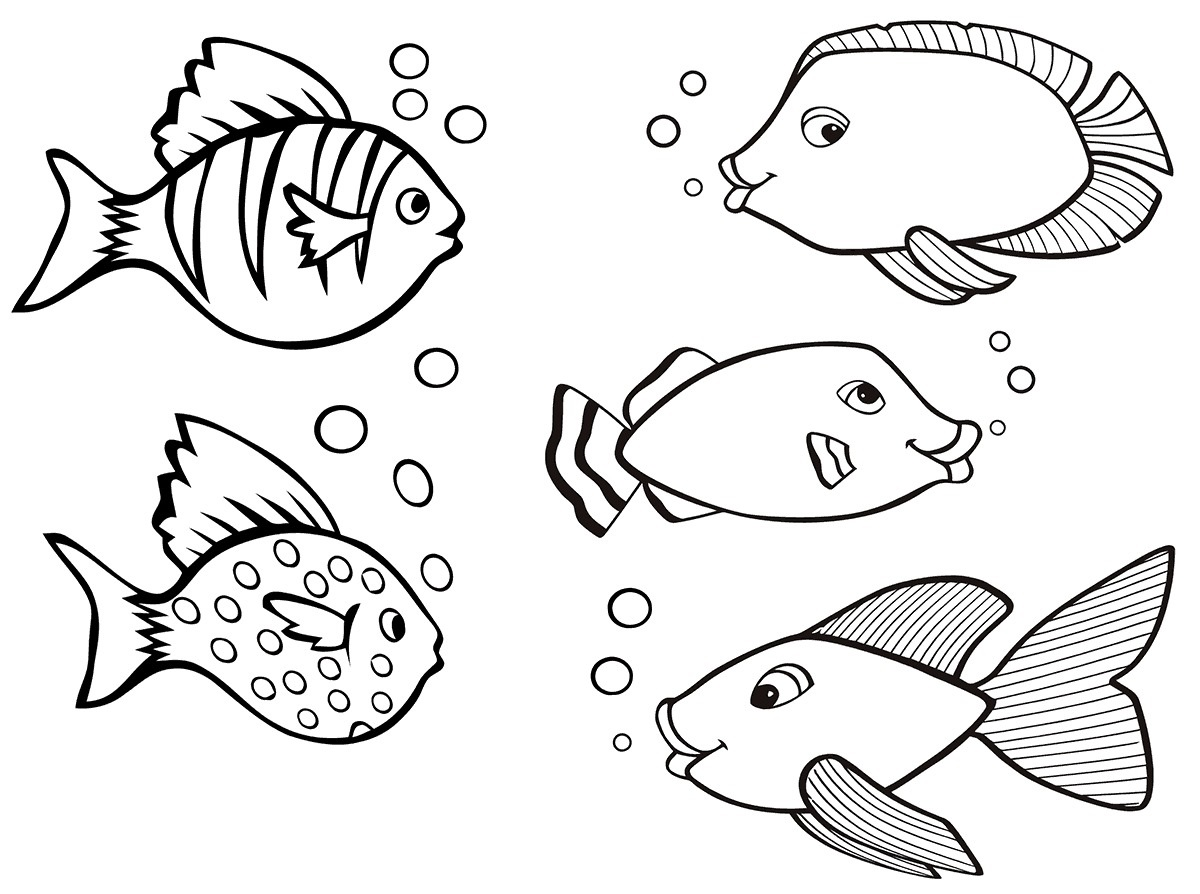
\includegraphics[width=0.4\textwidth]{tienkleinevisjes}
\end{intersong}
\beginsong{Tien kleine visjes}
\beginverse*
Tien kleine visjes, die gingen naar de zee,
't Is goed zei de moeder, maar ik ga niet mee. 
Ik blijf liever in de vieze, vuile sloot,
Want in de zee daar zitten haaien en die bijten je
Blub blub blubblubblubbblubblub, blub blub blubblubblubblubblub.
\endverse
\beginverse*
Negen kleine visjes … acht … zeven … … … …
\endverse
\beginverse*
één klein visje, dat ging naar de zee…
Want in de zee daar zitten haaien en die bijten je DOOD. 
\endverse
\endsong
\beginsong{Tinneke van Heule}
\beginverse*
Tinneke van Heule, ons maartje,
kan werken gelijk een paardje,
kan melken, kan mesten,
kan schuren gelijk de beste.
Tinneke van Heule, ons maartje,
staat hoog in de gunst van mijn vaartje
en als moederken haar prijst, dat mijn zuster er om krijst,
dan lach ik een beetj’ in mijn baardje.
\endverse
\beginchorus
Liever dan een vis die in de goudzee zwemt,
liever dan een vogel die geen sparen kent,
liever dan een fraule, Tinneke van Heule
Tinneke, ons maartje, in haar hemd. \rep{2}
\endchorus
\beginverse*
Tinneke heeft geld noch goedje, 
noch landeke, noch panneke, noch koetje,
noch huisje, noch kruisje,
noch een lappeke voor op mijn buisje.
Tinneke heeft geld noch goedje,
maar een hemel in haar lachen en haar grotje,
als zij trippelt naar de bron, met haar emmer in de zon,
en haar klompeken vast aan haar voetje.
\endverse
\beginverse*
Tinneke van Heule, mijn minneken,
op U staat mijn zoetste zinneken.
U lust ik, U kust’ ik, 
op uw harteken bouw en rust ik.
Tinneke van Heule, mijn minneken,
mijn poezelig dubbel kinneken,
leg uw handeken in de mijn, en een bruiloft zal het zijn,
van een boer en een schoon boerinneken.
\endverse
\endsong 
\beginsong{Toffe jongens}
\beginverse*
En dat we toffe jongens zijn dat willen wij weten,
Daarom komen wij, daarom komen wij,
En dat we toffe jongens zijn dat willen wij weten,
Daarom komen wij overal. 
Overal, overal , waar de meisjes zijn, waar de meisjes zijn,
Overal, overal, waar de meisjes zijn daar is het bal. 
\endverse
\endsong 
\beginsong{Tok Tok Tokketokketok}
\beginverse*
Tok tok, tokketokketok,
Zingen alle kippen,
Tok tok, tokketokketok,
In het kippenhok bom bom bom bom (volledig herhalen)
\endverse
\endsong 
\beginsong{Tom Dooley}
\beginchorus
Hang down your head, Tom Dooley,
hang down your head and cry.
Hang down your head, Tom Dooley,
poor boy, you’re born to die.
\endchorus
\beginverse*
I met her in the mountain,
and there I took her life.
I met her on the mountain,
and stabbed her with my knife.
\endverse
\beginverse*
This time tomorrow,
reckon where I’ll be.
If it hadn’t been for Grayson,
i’d been for Tennessee.
\endverse
\beginverse*
This time tomorrow,
reckon where I’ll be.
In some lonesome valley,
hanging on with oak tree.
\endverse
\endsong 
\beginsong{Trink, trink, Brüderlein trink}
\beginverse*
Das trinken, das soll man nicht lassen,
das trinken regiert doch die welt.
man soll auch der Menschen nicht hassen,
der stets eine Lage bestellt.
Ob bier, oder wein, ob champagner,
nur lasst uns beim trinken nicht prahlen.
Es trank der Champagner schon mancher,
und konn ihn nachher nicht bezahlen.
\endverse
\beginverse*
Trink, trink, Brüderlein trink,
lass toch die Sorgen zu hause.
Trink, trink, Brüderlein trink,
zieh doch die Stirn nicht zu grauss.
Meide den kummer und meide den Schmerz,
dan ist das leben ein Scherz.
\endverse
\endsong 
\begin{intersong}
    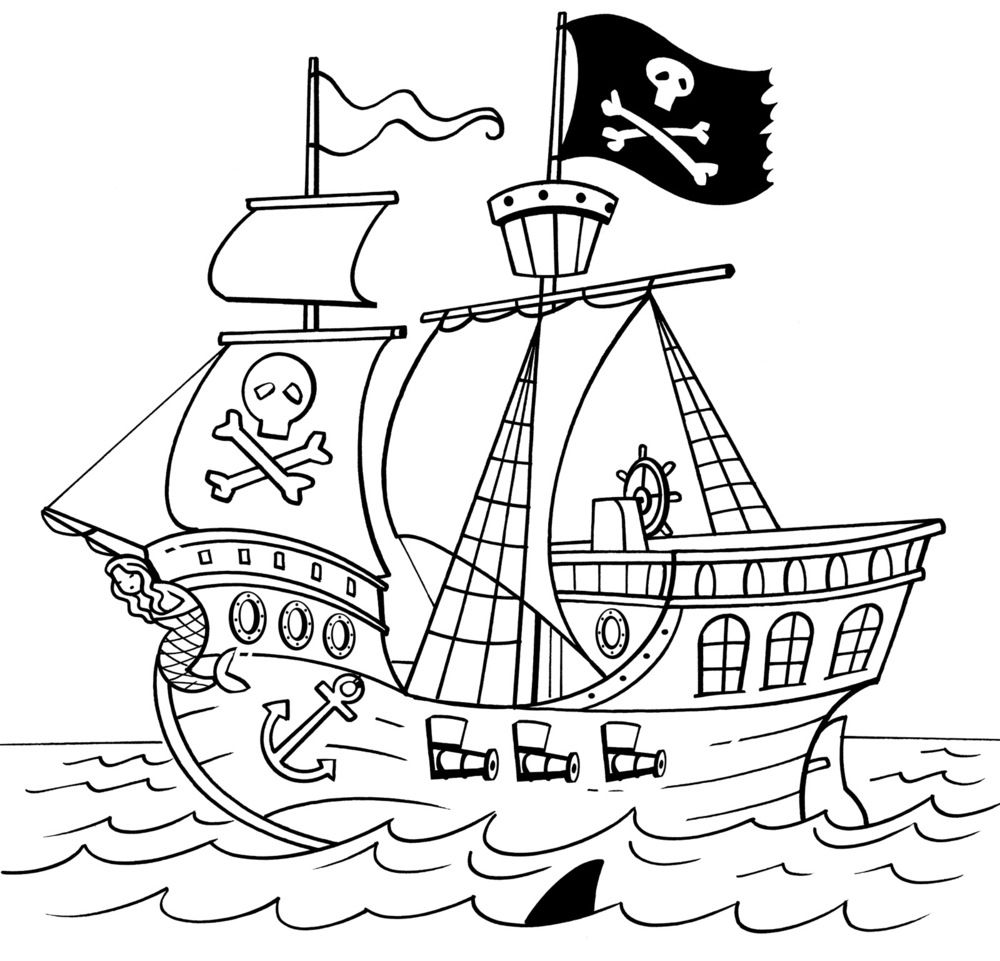
\includegraphics[width=0.4\textwidth]{triomfantelijkliedvandezilvervloot}
\end{intersong}
\beginsong{Triomfantelijk lied van de zilvervloot}
\beginverse*
Heb je van al gehoord van de Zilveren Vloot
De Zilveren Vloot van Spanje?
Die hadden veel Spaanse matten aan boord
En appeltjes van Oranje!
Piet Hein, Piet Hein,
Piet Hein zijn naam is klein,
Zijn daden bennen groot: (bis)
Die heeft gewonnen de Zilveren Vloot,
Die heeft gewonnen, gewonnen de Zilvervloot.
\endverse
\beginverse*
Zei toen niet Piet Hein met aalwarig woord:
"Wel jongetjes van Oranje,
Kom klim'reis aan dit en dat Spaanse boord
en rol met de matten van Spanje!"
Piet Hein, enz...
\endverse
\beginverse*
Klommen niet de jongens als katten in 't want
En vochten ze niet als leeuwen?
Ze maakten de Spanjers duchtig te schand
Tot Spanje klonk hun schreeuwen.
Piet Hein, enz…
\endverse
\beginverse*
Kwam er nu nog eenmaal zo'n Zilveren Vloot
Zeg, zou jullie nog zo kloppen?
Of zoudt gij u veilig buiten schoot
Maar stil in je hangmat stoppen?
"Wel Neerlands bloed,
Dat bloed heeft nog wel moed!
Al bennen we niet groot, (bis)
We zoùen winnen een Zilveren Vloot
We zoùen winnen, nog winnen een Zilvervloot!"
\endverse
\endsong
\beginsong{uit die blou}
\beginverse*
Uit die blou van onse hemel, uit die diepte van ons see,
Oor ons ewige gebergtes, waar die kranse antwoord gee,
Deur ons vér verlate vlaktes met die kreun van ossewa,
Ruis die stem van ons geliefde, van ons land Suid-Afrika.
Ons sal antwoord op jouw roepstem, ons sal offer wat jy vra,
Ons sal lewe, ons sal sterwe, ons vir jou Suid-Afrika.
\endverse
\beginverse*
In die merg van ons gebeente, in ons hart en siel en gees,
In ons roem op ons verlede, in ons hoop op wat zal wees,
In ons wil en werk en wandel, van on swieg tot aan ons graf,
Deel geen ander land ons liefde, trek geen ander trou ons af.
Vaderland! Ons sal die adel van jou naam met are dra:
Waar en trou, as Afrikaners - kinders van Suid-Afrika!
\endverse
\endsong 
\beginsong{Uw liederen zij klonken}
\beginverse*
Uw liederen zij klonken, tot ver in de hei,
Zij drongen door straten en stegen tot mij.
Uw dreunende stappen zijn verder gegaan,
Zo hebt gij uw taak in het leven verstaan.
\endverse
\beginchorus
Met heldere ogen, met kranige moed,
Bezien wij de plicht die strijden doet.
En alle verkenners, de lelie voorop.
Zij schrijden vooruit naar hogeren top
\endchorus
\beginverse*
En wijl gij marsjeerde, ben ik blijven staan,
De wereld zij lonkte niet verder te gaan.
Maar midden dien twijfel klonk plots weer een lied,
Gij roept uit de verten, ik weet wat gij bediedt.
\endverse
\beginverse*
En nu wil ik schrijden naast U in de rij,
Weer klinken mijn liedren tot ver in de hei.
En was ik een jongen die ’t leven begeert,
Dan heb ik het in uw rangen geleerd.
\endverse
\endsong
\beginsong{Welkom broeders}
\beginverse*
Welkom broeders, welkom broeders,
welkom broeders, gij allen hier vergaard.
Welkom broeders, welkom broeders,
welkom broeders, hier rond het vuur geschaard.
\endverse 
\beginverse*
kom en laat ons zingen gaan,
zingen gaan, zingen gaan,
kom en laat ons zingen gaan,
dra komt 't afscheid aan.
\endverse 
\endsong 
\beginsong{Vaar mee kameraad}
\beginverse*
Trek aan de riemen, wij varen,
flink op de maat van een lied.
Klieft onze boot door de baren,
weg alle zorgen en verdriet.
\endverse
\beginchorus
Ohé kameraad, ohé kameraad,
vaar mee kameraad, vaar mee kameraad.
De zeilen haal op, haal op.
De vlag in de top, in de top ! \rep{2}
\endchorus
\beginverse*
Zijn wij niet jong en vol leven,
wij vrezen regen noch zon.
Stormen, zij doen ons niet beven,
't druipende nat: "'k lach er om".
\endverse
\beginverse*
Dreigen de stormen van 't leven,
Vikings dan goed opgelet.
Volgt het parool u gegeven.
't Klinkt: "Sta je man, sta je wet !"
\endverse
\endsong
\beginsong{Vaarwel}
\beginverse*
Er moet nu toch vaarwel gezegd,
en voor altijd vaarwel.
Aan vriend en spel vaarwel gezegd,
en voor altijd vaarwel.
\endverse
\beginchorus
Wel neen, 't is geen vaarwel,
mijn broer, dra zien w’elkander weer.
In vreugd en in jolijt mijn broer,
zien wij elkaar weer.
\endchorus
\beginverse*
Leg allen trouw de vriendenhand,
in vriendenband tegaar.
en binde vast dees vriendenband,
ons harten bij elkaar.
\endverse
\beginverse*
En waar zo scouts verbonden zijn,
mag geen vaarwel gehoord.
Maar rond den lichten wachtvuurschijn,
“tot weerziens” zij ons woord.
\endverse
\beginverse*
Want God die uit de hemel zendt, zijn zegen op ons neer.
Brengt ons in zijne hemeltent,
eens bij elkaar weer.
\endverse
\endsong 
\begin{intersong}
    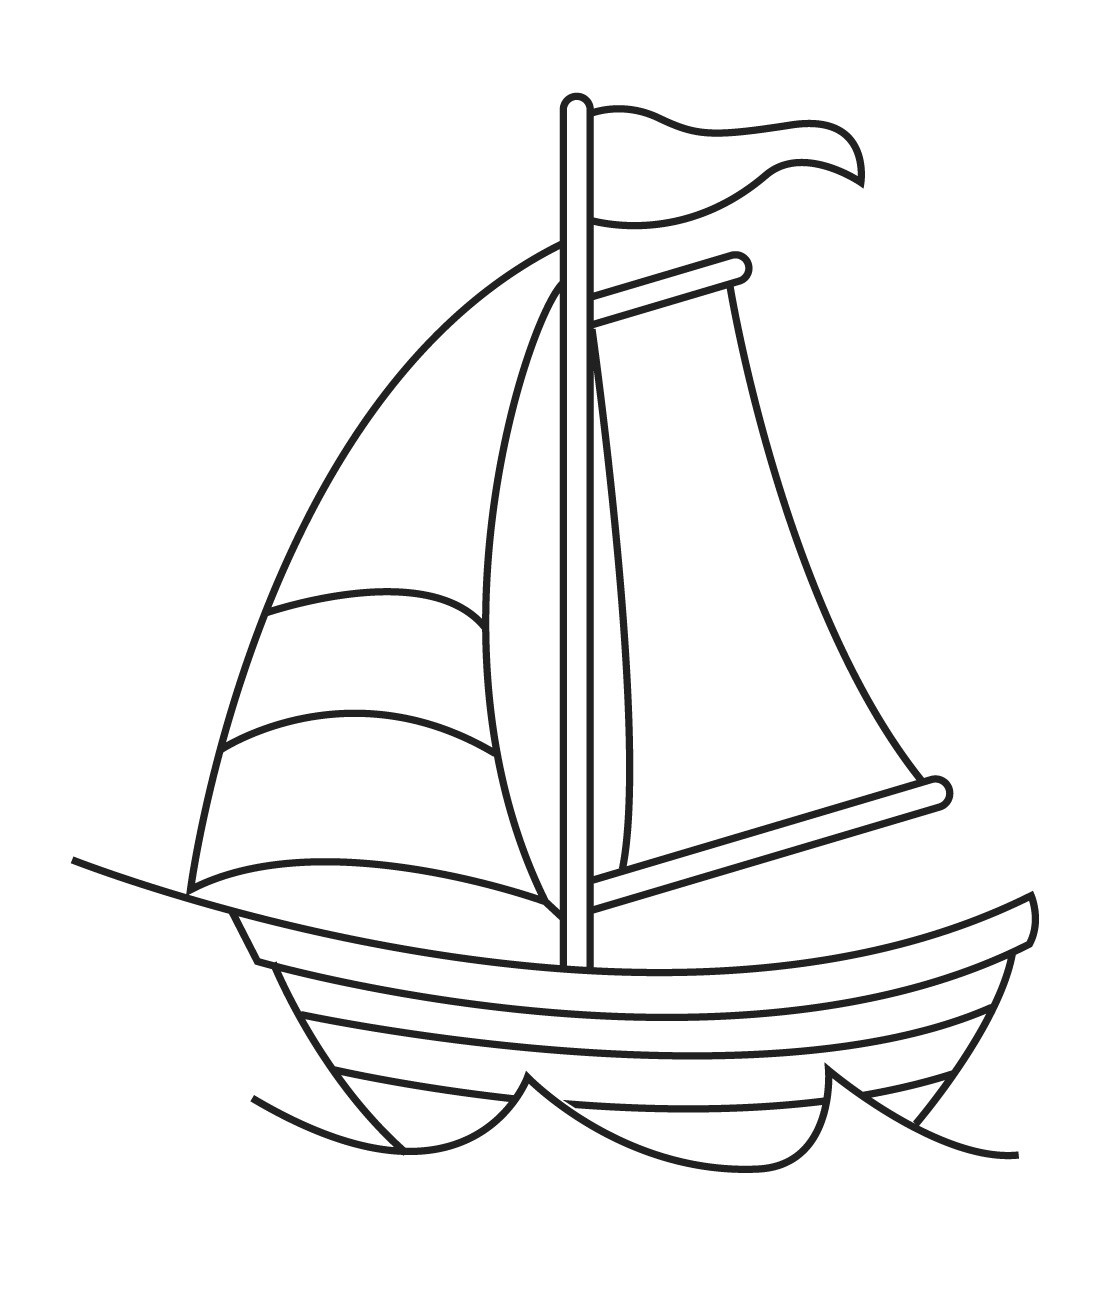
\includegraphics[width=0.4\textwidth]{vaarmaarmeekameraad}
\end{intersong}
\beginsong{Van voor naar achter}
\beginverse*
Een Nederlandse Amerikaan,
Die ziet men al van verre staan. \rep{2}
\endverse
\beginchorus
Van voor naar achter, van links naar rechts. \rep{4}
\endchorus
\beginverse*
Zijn hoofd lijkt wel op een varkenskop,
er staan maar amper drie haartjes op. \rep{2}
\endverse
\beginverse*
Zijn neus lijkt wel op een pingpongbal,
ik wou dat ik er mee spelen kan. \rep{2}
\endverse
\beginverse*
Zijn hemd lijkt wel op een prentenboek,
het hangt wel meters uit zijn broek. \rep{2}
\endverse
\beginverse*
Zijn buik lijkt wel op een luchtballon,
ik wou dat ik er in prikken kon. \rep{2}
\endverse
\endsong
\beginsong{Vlaanderen}
\beginverse*
't Zijn weiden als wiegende zeëen
Die groenen langs stroom en rivier.
Hier vredige dorpkens, daar steëen
Die rijzen net torens vol zwier;
't Zijn welige velden en wouden,
Of vlakten der heide vol rust.
O'k wil in mijn harte behouden
Die schoonheid, mijn oppersten lust.
\endverse
\beginchorus
Voor Vlaanderen, Vlaanderen,
Trille mijn harte vol geestdrift en vuur.
Mijn land is het land van de stille,
De vreedzame brede natuur.
\endchorus
\beginverse*
Uit beelden en doeken en zangen,
Uit al wat een kunstenaar schiep,
Straalt gij, als met tover omhangen,
Zo innig gevoeld en zo diep.
Gij spiegelt den aard uwer kindren,
Gij vindt in nun werken U weer;
Hoe zou mijn liefde vermindren,
U minnen wil ik meer en meer.
\endverse
\endsong
\beginsong{Vliegt de blauwvoet}
\beginverse
Een en een is twee \rep{2} Al de Franskiljons die moeten in de zee!
\endverse
\beginchorus
En vliegt de blauwvoet? \rep{3}Storm op zee!
En vliegt de blauwvoet? \rep{3}Storm op zee!
\endchorus
\beginverse
Twee en twee is vier \rep{2} al de Franskiljons in een vaatje bier!
\endverse
\beginverse
Drie en drie is zes \rep{2} al de Franskiljons in een tutterf les!
\endverse
\beginverse
Vier en vier is acht \rep{2} al de Franskiljons die moeten in de gracht!
\endverse
\beginverse
Vijf en vijf is tien \rep{2} al de Franskiljons die moeten in 't machien
\endverse
\beginchorus
En wij maar draaien \rep{2} tot z'er geel en zwart van zien!
En wij maar draaien \rep{2} tot z'er geel en zwart van zien!
\endchorus
\endsong
\beginsong{Vogeltje gij zijt gevangen}
\beginverse*
Vogeltje gij zijt gevangen,
In een kooitje zult gij hangen,
Gij blijft hier, gij blijft hier,
Lieve vogel gij blijft hier.
Handjes draaien, koekenbakken, vlaaien
Handjes draaien, koekenbakken, vis,
Ge kunt dat nie geloven, hoe lekker dat da is. 
\endverse
\endsong
\beginsong{Voor outer en heerd}
\beginverse*
Geen roekeloze wagers, stil volk dat zich beraadt,
Aleer het zijn belagers, aanheft te lijve gaat.
Zij wisten wat zij wilden, toen zij tot stout verweer. 
De pik of zeis optilden, of grepen naar 't geweer.
\endverse
\beginchorus
Voor outer en heerd,
Ongeknecht, onvereerd,
Voor outer en heerd,
Ongeknecht, onvereerd.
\endchorus
\beginverse*
Zij steunden op Oranje, de nederlanden één,
En juichten toen Brittanniës beloofde vloot verscheen.
Kloekmoeding in de gouwen van Diets Zuid-Nederland,
Zijn allen sterk en trouwe, gesprongen in den brand.
\endverse
\endsong
\beginsong{Vrolijke vrienden}
\beginchorus
Vrolijke, vrolijke vrienden,
Vrolijke vrienden, dat zijn wij \rep{2}.
\endchorus
\beginverse*
Als wij samen gaan kamperen,
In het bos of op de hei,
Dan klinkt het wel duizend keren,
Vrolijke vrienden dat zijn wij. 
\endverse
\beginverse*
's Morgens komt de zon ons wekken
en de vogels zingen blij
Dan is 't tijd dat wij gaan trekken
door de duinen, bos of hei. 
\endverse
\beginverse*
Twee of drie die koken 't eten
brengen lekk're dingen mee
Er is iets dat wij wel weten,
wie op kamp is eet voor twee! 
\endverse
\beginverse*
En gaat stil de avond komen,
zingen, dansen wij bij 't vuur
Tot wij in ons tent gaan dromen
in het late, late uur!
\endverse
\endsong
\beginsong{Waarwij eens als makkers streden}
\beginverse*
Waar wij eens als makker streden,
and’ren staan met jeugdig frisse kracht.
Daar waar wij niet verder schreden,
stormen zijn, terwijl de zege lacht.
\endverse
\beginchorus
Uw spoor is diep, ja diep,
in ons gedreven,
mijn lelievlag, mijn lelievlag,
en daarom blijf ik steeds,
uw beeld beleven,
wij zien ons weder als ik trouw zijn mag,
tot wij zien gloren, de nieuwe dag.
\endchorus
\beginverse*
Ginds omhoog daar droomt een sterre,
Brengt een groet aan die verdwenen zijn.
En hun lied klinkt steeds van verre,
stonden zij ook eenmaal aan ons zij.
\endverse
\endsong
\beginsong{We shall overcome}
\beginverse
We shall overcome, \rep{3} some day.
oh, deep in my hart, I do believe,
That we shall overcome some day.
\endverse
\beginverse
we'll walk hand in hand, \rep{3} some day.
\endverse
\beginverse
We are not afraid, \rep{3} today.
\endverse
\beginverse
We shall live in peace, \rep{3} some day.
\endverse
\beginverse
The truth will make us free,\rep{3} some day.
\endverse
\beginverse
We shall thers be, \rep{3} some day.
\endverse
\endsong
\beginsong{We stegen met een zucht }
\beginverse*
We stegen met een zucht,
Tot boven in de lucht,
We zaten zo gezellig in ons huisje,
We konden alles zien,
We hadden pret voor tien,
Leve de zeppelin.
\endverse
\endsong
\beginsong{Were di}
\beginverse*
Schoon is de jeugd die zelf zich eert, sterk als gedegen staal,
Vredig van aard, naar die zich weer vecht voor heur ideaal.
Were di kameraad. Were di kameraad,
Eerst te woord, dan ter daad,
\endverse
\beginchorus
Were di kameraad,
Were di waar ge zijt,
Were di sta bereid,
Were di waar het lot U ook leidt
Were di.
\endchorus
\beginverse*
Flink is de jeugd die durft, en wat heur behoort in recht
Nooit zich vergooit voor vreemde wil, taai om heur waarden vecht.
\endverse
\beginverse*
Rijk is de jeugd die denkt en strijdt om wat nog komen moet,
Kloek en beraden zich bereidt, harten en zielen hoedt.
\endverse
\endsong
\beginsong{Westerwalderlied}
\beginverse*
Heute wollen wier marchieren,
einen neuen March probieren,
auf dem schönen Westerwald,
ja, da pfeift der Wind so kalt.
\endverse
\beginverse*
Oh! Du schoner Westerwald,
ueber deine Höhen pfeift der Wind so kalt
jedoch der kleinste sonnenschein
dringt tief ins Herz hinein.
\endverse
\beginverse*
Und die Gretl und der Hanz,
gehen am sonntag gem zum Tanz,
weil das Tanzen Freude macht,
ja, daz Herz im Leibe lacht.
\endverse
\endsong
\beginsong{What shall we do with the drunken sailor}
\beginverse
What shall we do with the drunken sailor? \rep{3}
\endverse
\beginchorus
Early in the morning.
\endchorus
\beginverse
Hooray and up she rises, \rep{3}
\endverse
\beginverse
Put him in the long boat until he’s sober. \rep{3}
\endverse
\beginverse
Pull out the plug and wet him all over. \rep{3}
\endverse
\beginverse
Put him in the scuppers with a hose-pipe on him. \rep{3}
\endverse
\beginverse
Heave him by the leg in a running bowlin’. \rep{3}
\endverse
\beginverse
Tie him to the taffrail when she’s yard-arm under. \rep{3}
\endverse
\endsong
\beginsong{Wij zijn al bijeen}
\beginverse*
Wij zijn al’ bijeen, zotte kadullen, zotte kadullen
Wij zijn al’ bijeen , zotte kadullen ondereen.
Zou men nie meugen een pintje drinken,
Zonder daarom een dronkaard te zijn?
Zou men nie meugen een visje eten,
Zonder daarom een snoeper te zijn.
Zou men nie meugen eens vrolijk wezen,
Zou men nie meugen vrolijk zijn.
\endverse
\beginverse*
Wij zijn al’...
\endverse
\endsong
\beginsong{Woutertje}
\beginverse*
Ik zag hem voor’t eerst op de mat in de gang
Ik zei: “Goeiemorgen, ben jij hier al lang?”
Hij zei: “Nou ik denk een minuutje of vijf.”
“Maar ’k vind je wel aardig, ik denk dat ik blijf.”
\endverse
\beginchorus
Woutertje, Woutertje wiezewiezewiezewoep
Piepklein kaboutertje, kom als ik roep. \rep{2}
\endchorus
\beginverse*
Ik heb hem al jaren en nooit geeft ie last.
Hij woont in een trommeltje onder de kast.
En 's morgens om zeven uur maakt ie geluid.
Dan roept ie om eten en wil ie er uit.
\endverse
\beginverse*
Hij is reuze aardig en w’hebben veel pret.
maar 's avonds om zeven uur wil ie naar bed.
Hij trekt zijn pyjamaatje aan van katoen.
Dan rolt ie zijn baard op en krijgt nog een zoen.
\endverse
\endsong
\begin{intersong}
    
\includegraphics[width=0.4\textwidth]{youaremysunshine}
\end{intersong}
\beginsong{You are my sunshine}
\beginverse*
You are my sunshine
My only sunshine
You make me happy, when skies are gray
You’ll never know dear, how much I love you
Please don’t take my sunshine away.
\endverse
\beginverse*
The other night dear,
When I was sleeping
I dreamed I held you in my arms
But when I waked up, I was mistaken
So I laid down my head and I cried.
\endverse
\endsong
\beginsong{Zeeroverslied}
\beginverse*
De machtigste koning van storm en van wind 
Is de arend geweldig en groot. 
De vogels sidderen en vluchten van angst 
Voor zijn snavel en klauwende poot! 
Als de leeuw verheft zijn gebrul des nachts 
Dan verschrikt hij de dieren er mee 
Ja we zij de heersers der aard,
De koningen van de zee.
\endverse
\beginchorus
Tiralala, tiralala-tiralala, tiralala hoi, hoi! 
Ja we zijn de heersers der aard 
De koningen van de zee! 
\endchorus
\beginverse*
Verschijnt er een schip op den oceaan 
Dan juichen wij luide en wild 
Ons trotse schip als een pijl uit den boog 
Vliegt terstonds door de wateren zilt, 
De koopman wordt bang en hij siddert van angst 
De matrozen verwenschen dien dag 
En daar klimt de mast langs omhoog 
Onze bloedrode zeeroversvlag!
\endverse
\beginverse*
Wij werpen ons op het vijandige schip 
Als een weggeslingerde speer 
De kanonnen dreunen, ’t geweer knalt rondom
En de enterbijl hakt keer op keer
En reeds zinkt de vlag van den vijand omlaag. Overwinningsgeroep alom Lang leve de bruisende zee! Lang leve de zeeroverij. 
\endverse
\beginverse*
En is zo gewonnen het laatste gevecht, 
En de laatste overwinning behaald, 
Dan fluks onze wrakkige schuit naar den 
Duivel gestuurd en ter helle gedaald 
En als satan dan onze wil niet doet Ai- dan roosteren wij hem eens fel 
Want wij zijn de heersers der aard 
En wij willen ’t ook zijn in de hel!
\endverse
\endsong
\beginsong{Zeg kwezelken, wilde gij dansen?}
\beginverse*
Zeg kwezelken, wilde gij dansen?
Ik zal u geven een ei.
Wel neen ik, zei dat kwezelken,
Van dansen ben ik vrij.
'k En kan niet dansen,
'k En mag niet dansen:
Dansen is onze regel niet,
Begijntjes en kwezelkens dansen niet.
\endverse
\beginverse*
Zeg kwezelken, wilde gij dansen?
Ik zal u geven een koe.
Wel neen ik, zei dat kwezelken,
Van dansen word ik te moe.
'k En kan niet …
\endverse
\beginverse*
Zeg kwezelken, wilde gij
dansen?
Ik zal u geven een paard.
Wel neen ik, zei dat kwezelken,
't En is mij 't dansen niet waard
'k En kan niet…
\endverse
\beginverse*
Zeg kwezelken, wilde gij dansen,
Ik zal u geven een man.
Wel ja ik, zei dat kwezelken,
'k Zal ai doen wat ik kan.
Ik kan wel dansen,
Ik mag wel dansen:
Dansen is onze regel wel,
Begijntjes en kwezelkens dansen wel.
\endverse
\endsong
\beginsong{Zeven dagen lang}
\beginverse*
Wat zullen we drinken, zeven dagen lang?
wat zullen we drinken, wat een dorst. \rep{2}
\endverse
\beginverse*
Er is genoeg voor iedereen,
Dus drinken we samen, sla het vat maar aan,
Ja drinken we samen, niet alleen! \rep{2}
\endverse
\beginverse*
Dan zullen we werken, zeven dagen lang,
Dan zullen we werken, voor elkaar. \rep{2}
\endverse
\beginverse*
Dan is er werk voor iedereen, 
Dus werken we samen, zeven dagen lang, 
Ja werken we samen, niet alleen! \rep{2}
\endverse
\beginverse*
Eerst moeten we vechten, niemand weet hoelang,
Eerst moeten we vechten voor ons belang. \rep{2}
\endverse
\beginverse*
Voor het geluk van iedereen,
Dus vechten we samen, samen staan we sterk,
Ja vechten we samen, niet alleen! \rep{2}
\endverse
\endsong
\beginsong{Zingen is een ding}
\beginchorus
Zingen is een ding,
Dat maakt een mens zo flink,
Zingen is een ding dat ons bijeen houdt.
Al zijn we nog zo oud,
En zoveel jaren scout,
Zingen is een ding dat ons bijeen houdt. 
\endchorus
\beginverse*
Bij 't kraaien van de haan,
Stappen wij al op de baan,
De knapzak op de rug en blote knieën.
Dan zoeken wij in’t bos,
Naar het zachtste plekje mos. 
Intusen zingen wij er dan maar flink op los. 
\endverse
\beginverse*
Zo rond het middaguur,
staan de pannekes op het vuur,
en liggen de kotelettekes te braden.
Gebeurt het impesant,
dat den boel is aangebrand.
Dan scheppen we het diner maar onder het zand.
\endverse
\endsong
\beginsong{Zingend op weg}
\beginverse*
Na korten overleg, tralalalalala,
Zijn wij weer eens op weg, tralalalalala,
Eenieder kijkt ons aan, ralalalalala,
Als wij op uitstap gaan tralalalalala.
\endverse
\beginverse*
Wij volgen 't rechte spoor,
En zingen dan maar door,
Vol levenslust en moed,
Dat doet ons hartje goed.
\endverse
\beginverse*
Ja, zingen doen wij graag,
Bijzonderlijk vandaag,
Wij zingen laag en hoog,
Totdat ons keel is droog.
\endverse
\beginverse*
Zijn wij eens oud en grijs,
Dan gaan wij nog op reis,
En zingen 't scoutenlied,
En zwijgen doen wij niet.
\endverse
\beginverse*
Zo wordt ons leven lang,
Een blijde jubelzang,
Zo gaan wij eenmaal weer,
Al ziengend naar ons Heer.
\endverse
\endsong
\begin{intersong}
    
\includegraphics[width=0.4\textwidth]{zwartbruinisdehazelnoot}
\end{intersong}
\beginsong{Zwartbruin is de hazelnoot}
\beginverse*
Zwartbruin is de hazelnoot
zwartbruin ook ben ik, ja, ik
zwartbruin meet eenieder zijn
die zijn wil zoals ik
\endverse
\beginchorus
Holdrio, juvi juvi je hahaha
holdrio, juvi juvi je hahaha
holdrio, juvi juvi je hahaha
holdrio, juvi juvi je
juvi juvi je hahaha
juvi juvi je hahaha
juvi juvi je hahaha
Juvi juvi je
\endchorus
\beginverse*
koffie op het kamp zwartbruin
want zwartbruin ben ik, ja, ik
als de kok het toch verprutst
krijg je koffiedik
\endverse
\beginverse*
zwartbruin is ons rantsoen brood
oversopt met surrogaat
maar dat smaakt toch even goed
als men op kamping gaat
\endverse
\endsong




\end{songs}

\showindex[2]{Inhoudstafel}{mainindex}

\end{document}
